\documentclass[%
thesis=student,% bachlor's or master's thesis
coverpage=false,% do not print an extra cover page
titlepage=false,% do not print an extra title page
headmarks=true, % headmarks can be switched on or off
german,% or `english`
font=libertine, % use `libertine` font; alternatives: `helvet` / `palatino` / `times`
math=newpxtx, % math font `newpxtx`; alternatives: `ams`, `pxtx`
BCOR=5mm,% binding correction - adapt accordingly
coverBCOR=11mm% binding correction for the cover - adapt accordingly
]{tumbook}
%--------------------------------------------------------

%--------PACKAGES----------------------------------------

%--------------------------------------------------------
\usepackage{tikz}
\usetikzlibrary{arrows.meta, positioning, calc, automata, shapes.geometric}
\usepackage{pgfplots}
\usepackage{float}
\usepackage{lipsum}
\usepackage{algorithm2e}
\usepackage{booktabs}% for more beautiful tables
\usepackage{cleveref}% intelligent references
\usepackage{eso-pic}
\usepackage{diffcoeff}
\usepackage{amsthm}
\usepackage{amsmath}

% Laden von Paketen und Festlegen von Optionen
%\PassOptionsToPackage{autostyle=true,german=quotes}{csquotes}
%\PassOptionsToPackage{backend=biber,style=numeric}{biblatex}

% Pakete laden
\usepackage{csquotes}
%\usepackage{biblatex}
\usepackage[backend=biber,style=alphabetic,citestyle=authoryear]{biblatex}
\addbibresource{literature.bib} % Ihre .bib-Datei


\usepackage{listings}
\usepackage{xcolor}

\lstset{
	language=Python,
	basicstyle=\ttfamily\small,
	keywordstyle=\color{blue},
	commentstyle=\color{gray},
	stringstyle=\color{green},
	numbers=left,
	numberstyle=\tiny\color{gray},
	stepnumber=1,
	numbersep=5pt,
	showstringspaces=false,
	breaklines=true,
	frame=lines,
	captionpos=b,
	tabsize=2,
	morekeywords={self}
}
%-------------------------------------------------------------------------------
\newtheoremstyle{break}
{\topsep}   % Platz oberhalb
{\topsep}   % Platz unterhalb
{\itshape}  % Schriftart im Textkörper
{0pt}       % Einzug (keiner)
{\bfseries} % Schriftart im Kopf
{.}         % Punkt nach Theorem-Name
{\newline}  % Zeilenabstand nach Theorem-Name
{}          % Zusätzliche Spezifikation


\theoremstyle{break}
\newtheorem{definition}{Definition}[section]
\newtheorem{theorem}[definition]{Satz}

% Command to include background image
\newcommand\BackgroundPic{
	\put(0,0){
		\parbox[b][\paperheight]{\paperwidth}{
			\vfill
			\centering
			
\includegraphics[width=\paperwidth,height=\paperheight,keepaspectratio]{deckblatt.pdf}
			\vfill
}}}

% Command to include logo image
\newcommand\LogoPic{
	\put(\LenToUnit{0.7\paperwidth},\LenToUnit{0.75\paperheight}){
		\parbox[b][\paperheight]{\paperwidth}{
			\vfill
			\raggedleft
			
\includegraphics[width=0.4\textwidth]{Logo_Uni_alt.pdf}
			\vfill
}}}
%-------------------------------------------------------------------------------
\title{Dies ist der Titel der Arbeit}
\author{Max Mustermann}
\date{\today}
\pagenumbering{arabic}

%-------------------------------------------------------------------------------
\begin{document}
	
\pagenumbering{arabic}
% Title Page
\begin{titlepage}
	\AddToShipoutPicture*{\BackgroundPic}
	\AddToShipoutPicture*{\LogoPic}
	\centering
	\vspace*{1cm}
	
	\vfill
	
	\textsc{\LARGE Albert-Ludwigs-Universität Freiburg}\\[1.5cm]
	
	\textsc{\Large Bachelorarbeit}\\[0.5cm]
	
	\rule{\linewidth}{0.5mm} \\[0.4cm]
	{ \huge \bfseries Verzerrung der Inferenz bei Verwendung gemischter Modelle in latenten Repräsentationen}\\[0.4cm]
	\rule{\linewidth}{0.5mm} \\[1.5cm]
	
	\begin{minipage}{0.4\textwidth}
		\begin{flushleft} \large
			\emph{Autor:}\\
			Yannick Bantel \\
			\vspace{5pt}
			\emph{Professor:} \\
			Prof. Dr. Harald Binder \\
			\vspace{5pt}
			\emph{Betreuer:} \\
			Clemens Schächter\\

		\end{flushleft}
	\end{minipage}
	\begin{minipage}{0.4\textwidth}
		\begin{flushright} \large
			\emph{Abgabedatum:} \\
			\today
		\end{flushright}
	\end{minipage}\\[3cm]
	
	\begin{tikzpicture}[remember picture, overlay]
		\node[anchor=south east, xshift=-2cm, yshift=3cm] at (current page.south east) {
			
\includegraphics[width=0.2\textwidth]{Logo_Uni_alt.pdf}
		};
	\end{tikzpicture}
	
	\vfill
	

	
\end{titlepage}
\frontmatter
\pagenumbering{arabic}
%\maketitle

\cleardoublepage{}

\tableofcontents

\cleardoublepage{}

\section*{Abstract}
This thesis examines the potential for bias in inference when utilising mixed models in latent representations. The research primarily focuses on the application of Variational Autoencoders (VAE) combined with mixed models to analyse high-dimensional medical datasets. The study investigates the extent to which inference results may be biased and evaluates the robustness of the models used. The objective of this study is to examine the likelihood-ratio test statistics and compare them across different model configurations in order to gain insights into the reliability of using VAEs in conjunction with mixed models for statistical analysis.
\mainmatter{}
\pagenumbering{arabic}
%%---------------EINLEITUNG--------------------------------------------------
\chapter{Einleitung}
Die Anwendung gemischter Modelle zur Analyse und Verarbeitung komplexer Datenstrukturen stellt in vielen wissenschaftlichen und industriellen Bereichen eine Herausforderung dar und hat in den letzten Jahren stark an Bedeutung gewonnen. Insbesondere in der medizinischen Datenwissenschaft und maschinellen Lernverfahren sind Datensätze oft durch hohe Dimensionen und komplexe Strukturen gekennzeichnet, was die Analyse und Interpretation erschwert. Die Anwendung gemischter Modelle in latenten Repräsentationen könnte eine vielversprechende Methode sein, um die Handhabung solcher Datenstrukturen zu erleichtern.\\
\\
Gemischte Modelle ermöglichen 
es komplexe Datenstrukturen zu modellieren, in dem sie feste und zufällige Effekte kombinieren und so die Variabilität in den Daten besser abbilden und präzisere Vorhersagen ermöglichen. Allerdings bleibt die Handhabung hochdimensionaler Datenstrukturen sowohl rechnerisch intensiv als auch konzeptionell schwierig.\\
\\
Um diese Probleme zu behandeln wendet man gemischte Modelle  in latenten Repräsentationen an, um die dimensionsreduzierte Darstellung im latenten Raum auszunutzen. Latente Repräsentationen sind niedrigdimensionale Darstellungen der tatsächlichen Daten, die die wesentlichen Informationen und Merkmale beibehalten. Eine vielversprechende Methode zur Erstellung solcher latenten Repräsentationen ist der Variational Autoencoder (VAE). VAEs sind generative Modelle, die hochdimensionale Daten in einen niedrigdimensionalen latenten Raum transformieren, um die zugrunde liegenden Struktur zu erfassen und neue Daten zu generieren, die ähnliche Merkmale wie die Trainingsdaten aufweisen. Sie sind eine verbesserte Erweiterung der herkömmlichen Autoencoder. Durch die Reduktion der Dimension der Datensätze wird die Handhabung und Analyse erheblich vereinfacht, ohne wesentliche Informationen zu verlieren. \\
\\
Allerdings können solche Anwendungen eine Verzerrung der Inferenz verursachen.
Verzerrung in der Inferenz kann die Genauigkeit und Zuverlässigkeit von Schlussfolgerungen erheblich beeinträchtigen, was in vielen Bereichen, wie der medizinischen Diagnostik, schwerwiegende Konsequenzen haben kann. Daher ist es von großer Bedeutung, die Ursachen und Auswirkungen dieser Verzerrungen zu verstehen und Methoden zu ihrer Minimierung zu entwickeln. Um in der Zukunft die Vorteile der Anwendung gemischter Modelle in latenten Repräsentationen auszunutzen, wird in dieser Arbeit die womöglich auftretende Verzerrung der Inferenz analysiert und quantifiziert. Besonders wird analysiert, wie die Kombination von VAE und gemischten Modellen die statistischen Eigenschaften der Inferenz beeinflusst. \\
\\
Im ersten Teil der Arbeit, dem Kapitel "Theoretische Grundlagen",  werden die theoretischen Aspekte von Variational Autoencodern  und gemischten Modellen erläutert. Die Architektur und das Training von Variational Autoencodern wird detailliert beschrieben, um ein tiefes Verständnis ihrer Funktionsweise zu vermitteln.\\
\\
Anschließend werden gemischte Modelle beschrieben, welche besonders nützlich bei der Analyse von Längsschnitt- und Cluster-Daten sind, wie sie in der Medizin, den Sozialwissenschaften und der Ökonomie häufig vorkommen. Ein zentrales Element der gemischten Modelle ist die Likelihood-Inferenz, bei der die Parameter durch Maximum-Likelihood-Schätzung bestimmt werden. Zudem werden die nötigen Kenntnisse für die späteren Testverfahren geschaffen \\
\\
Im empirischen Teil der Arbeit wird ein komplexer,  medizinischer Datensatz verwendet, um die Verzerrung der Inferenz bei der Anwendung gemischter Modelle auf latente Repräsentationen zu untersuchen. Die Analyse basiert auf der Likelihood-Ratio-Test Statistik, die zwischen einem vollständigen und einem reduzierten gemischten Modell unterscheidet. Durch wiederholtes Training und Evaluierung dieser Modelle auf der latenten Datenwolke des Variational Autoencoders wird die Verzerrung quantifiziert und bewertet.\\
\\
Die Ergebnisse dieser Untersuchung tragen dazu bei, die Zuverlässigkeit von Inferenzmethoden in Kombination mit VAEs zu bewerten und liefern wertvolle Erkenntnisse für die praktische Anwendung solcher Modelle. Abschließend werden die Implikationen der Ergebnisse diskutiert und Empfehlungen für zukünftige Forschungen gegeben.\\
\\

%%-------------THEORETISCHE-GRUNDLAGEN---------------------------------------
\chapter{Theoretische Grundlagen}
Im Vorfeld der Erörterung der Methodik dieser Arbeit ist eine theoretische Aufarbeitung der behandelten Themen unabdingbar. Dieses Kapitel widmet sich den theoretischen Grundlagen, die für das Verständnis und die Analyse von Verzerrungen in der Inferenz erforderlich sind, wenn gemischte Modelle in latenten Repräsentationen zum Einsatz kommen.\\
\\
Das vorliegende Kapitel beginnt mit einer detaillierten Einführung in Variational Autoencoder (VAE). VAEs sind generative Modelle, die es ermöglichen, hochdimensionale Daten in niedrigdimensionale latente Repräsentationen zu überführen. Die Modelle reduzieren die Komplexität der Daten und sind in der Lage, sowohl die zugrunde liegende Struktur der Daten zu erfassen als auch neue Daten zu generieren, die ähnliche Merkmale wie die Trainingsdaten aufweisen. Die Architektur und das Training von VAEs werden detailliert beschrieben, um ein fundiertes Verständnis ihrer Funktionsweise zu vermitteln.\\
\\
Im zweiten Teil des Kapitels erfolgt eine Behandlung von gemischten Modellen. Die Modelle kombinieren feste und zufällige Effekte, um die Variabilität in den Daten zu erfassen. Ihre Anwendung ist insbesondere bei der Analyse longitudinaler und Cluster-Daten von Vorteil, wie sie in den Bereichen Medizin, Sozialwissenschaften und Ökonomie häufig auftreten. Die Grundlagen gemischter Modelle, einschließlich der Annahmen und mathematischen Formulierungen, werden ausführlich erörtert.\\
\\
Ein zentrales Element der theoretischen Grundlagen ist die Likelihood-Inferenz. Im Folgenden wird die Schätzung der Parameter von gemischten Modellen unter Verwendung der Maximum-Likelihood-Methode erörtert. Es wird insbesondere dargelegt, wie die Likelihood-Funktion zur Schätzung der festen und zufälligen Effekte maximiert wird und wie der Likelihood-Ratio-Test (LRT) zur Evaluierung der Modelle zum Einsatz kommt. Der Likelihood-Ratio-Test (LRT) erlaubt die Bestimmung der Signifikanz zusätzlicher Parameter sowie die Identifikation potenzieller Verzerrungen in der Inferenz.\\
\\
In diesem Kapitel wird die theoretische Basis für die nachfolgenden empirischen Untersuchungen dargelegt. Der vorliegende Abschnitt bietet eine umfassende Darstellung der relevanten Methoden und Konzepte, welche erforderlich sind, um die Verzerrung der Inferenz bei der Verwendung gemischter Modelle in latenten Repräsentationen zu verstehen und zu analysieren.\\

%----------------------------------------------------------------------------

%-----------------------VARIATIONAL-AUTOENCODER------------------------------

%----------------------------------------------------------------------------
\section{Einführung in Variational Autoencoder (VAE)}
Die Anwendung der gemischten Modelle auf einer latenten Repräsentation erfolgt,wie bereits erwähnt, mittels Variational Autoencoder (VAE).
Variational Autoencoder sind für die Modellierung latenter Repräsentationen von großem Interesse, da sie hochdimensionale Datensätze mit Hilfe ihres Encoders im latenten Raum  niedrigdimensional darstellen können. Dies reduziert die Komplexität der Modellierung und ermöglicht es, gemischte Modelle effizienter und genauer zu betreiben. Sie sind generative Modelle, welche versuchen die zugrunde liegende Struktur der Inputdaten x im latenten Raum zu modellieren.\\
Im Gegensatz zu herkömmlichen Autoencodern ist der VAE in der Lage, nicht nur den Eingabedatensatz zu rekonstruieren, sondern auch neue Inhalte, die ähnliche Merkmale wie die Trainingsdaten aufweisen, zu generieren. Dies wird durch die verbesserte Repräsentation ermöglicht (vgl. \cite{bigdata-insider-vae}). Insbesondere wird der latente Raum nicht wie bei normalen Autoencoder durch feste Punkte modellieret, wie es in Abbildung \ref{fig:vae} dargestellt ist, sondern in der Erweiterung VAE durch eine Wahrscheinlichkeitsverteilung (Normalverteilung).
\begin{figure}
	\centering
	\begin{tikzpicture}[auto, thick, node distance=2cm, >=stealth]
		
		% Define styles
		\tikzstyle{latent} = [rectangle, draw, fill=blue!20, text centered, minimum width=1cm, minimum height=2cm]
		\tikzstyle{input} = [rectangle, draw, fill=yellow!20,text centered, minimum width=1cm, minimum height=3cm]
		\tikzstyle{output} = [rectangle,draw, fill=yellow!20, text centered, minimum width=1cm, minimum height=3cm]
		
		% Nodes
		\node[input, name=input] (input) {x};
		\node[latent, right of=input, node distance=6cm, minimum width=1cm, minimum height=2cm] (z) {$z$};
		\node[output, right of=z, node distance=6cm] (output) {$\hat{x}$};
		
		% Custom trapezoids for encoder and decoder
		\draw[fill=gray!20] (3,2) -- (3,-2) -- (5,-1) -- (5,1) -- cycle;
		\node at (3.75, 0) {Encoder};
		
		\draw[fill=green!20] (7,1) -- (7,-1) -- (9,-2) -- (9,2) -- cycle;
		\node at (8, 0) {Decoder};
		
		% Arrows
		\draw[->] (input.east) -- (2.75,0);
		\draw[->] (5,0) -- (z.west);
		\draw[->] (z.east) -- (7,0);
		\draw[->] (9,0) -- (output.west);
		
		% Labels
		\node[above of=input, node distance=2cm] {Input};
		\node[above of=z, node distance=1.5cm] {Latent Space};
		\node[above of=output, node distance=2cm] {Reconstructed Data};
		
		% Additional Text
		\draw[->, thick] (output.south) |- ++(0, -2.5cm) -| (input.south);
		\node[below of=z, node distance=3.5cm, text width=6cm, align=center] {Reconstruction Loss};
		
		
	\end{tikzpicture}
	\caption{Aufbau eines herkömmlichen Autoencoders}
	\label{fig:autoencoder}
\end{figure}
\subsection{Strucktur des VAEs}
Die Architektur eines VAE basiert auf zwei neuronalen Netzwerken (einem Encoder Modell und einem Decoder Modell). Der Encoder ist ein neuroanles Netzwerk, das die hochdimensionalen Eingabedaten x durch mehrere Schichten hindurch in eine niedrigdimensionale latente Repräsentation z transformiert. Diese Transformation ermöglicht es, die zugrunde liegende Struktur der Daten zu erfassen und in einer komprimierten Form darzustellen.\\
Die latenten Variablen werden als Verteilung in Form eines Mittelwerts $\mu$ und einer Standardabweichung $\sigma$ kodiert. Der Decoder transformiert die latenten Daten so genau wie möglich zurück in die ursprünglichen Eingabedaten. Dies ermöglicht es, neue Datenpunkte zu generieren, die ähnliche Eigenschaften wie die Trainingsdaten aufweisen. Beide Modelle bestehen jeweils aus mehreren neuronalen Schichten, die jeweils die Transformation durchführen und lernen die wesentlichen Merkmale der Eingabedaten zu extrahieren und eine komprimierte Version dieser Daten zu erzeugen.\\
\\
\begin{figure}
	\centering
	
	\begin{tikzpicture}[auto, thick, node distance=2cm, >=stealth]
		
		% Define block styles
		\tikzstyle{block} = [trapezium, trapezium left angle=70, trapezium right angle=110, minimum height=3cm, draw, fill=gray!20, text centered]
		\tikzstyle{block2} = [trapezium, trapezium left angle=110, trapezium right angle=70, minimum height=3cm, draw, fill=green!20, text centered]
		\tikzstyle{square} = [rectangle, draw, fill=red!20, minimum size=1.5cm, text centered]
		\tikzstyle{latent} = [rectangle, draw, fill=blue!20, minimum size=1.5cm, text centered]
		
		% Nodes		
		\node[rectangle, draw, fill=yellow!20, minimum height=3cm, minimum width=1cm, text centered] (input) {$\mathbf{x}$};
		\draw[fill=gray!20] (1,2) -- (1,-2) -- (3,-1) -- (3,1) -- cycle;
		\node[right of=input, node distance=2cm] (encoder) {$q_{\phi}(z \mid x)$};
		\node[square, right of=encoder, node distance=2.5cm] (mu) {$\mu$};
		\node[square, below of=mu, node distance=2cm] (sigma) {$\sigma$};
		\node[latent, right of=mu, node distance=2cm] (z) {$\mathbf{z}$};
		\draw[fill=green!20] (8,1) -- (8,-1) -- (10,-2) -- (10,2) -- cycle;
		\node[right of=z, node distance=2.5cm] (decoder) { $p_{\theta}(x \mid z)$};	
		\node[rectangle, draw, fill=yellow!20, minimum height=3cm, minimum width=1cm, text centered, right of=decoder, node distance=3cm] (output) {$\hat{\mathbf{x}}$};
		
		
		
		% Arrows
		\draw[->] (input) -- (1,0);
		\draw[->] (3,0) -- (mu);
		\draw[->] (3,0) -- (sigma);
		\draw[->] (mu) -- (z);
		\draw[->] (sigma) -- (z);
		\draw[->] (z) -- (8,0);
		\draw[->] (10,0) -- (output);
		
		% Labels
		\node[above of=input, node distance=1.75cm] {Input Data};
		\node[above of=encoder, node distance=0.8cm] {Encoder};
		\node[above of=z, node distance=1cm] {Latenter Raum};
		\node[above of=decoder, node distance=0.8cm] {Decoder};
		\node[above of=output, node distance=1.75cm] {Reconstructed Data};

        \node[above of=mu, node distance=1.2cm] {Mittelwert};
		\node[below of=sigma, node distance=1.2cm] {Standardabweichung};
		
		% Additional Text
		\draw[->, thick] (input.south) |- ++(0, -2.5cm) -| (output.south);
		\node[below of=encoder, node distance=4.5cm, text width=6cm, align=center] {Reconstruction Loss + KL-Divergenz};
		
	\end{tikzpicture}
	\caption{Darstellung der Architektur eines Variational Autoencoders (VAE)}
	\label{fig:vae}
\end{figure}
\\
\textbf{Latenter Raum}\\
Variablen, die man nicht direkt messen kann, demnach nicht Teil des erhaltenen Datensatzes sind, bezeichnet man als latente Variablen. Sie werden erst mithilfe der gegebenen Daten erschlossen und ergeben im Verbund den latenten Raum.\\
Im VAE werden die latenten Variablen z aus der prior-Verteilung $p(z)$ gezogen, welche eine multivariate Normalverteilung $p(z) = \mathcal{N}(0,I) $ ist. Die latenten Daten sind der Output aus dem Encoder Modell, welches die  approximierte posterior Verteilung $q_\phi(z|x)$ parametrisiert, wobei $\phi$ der Parametervektor des Encoders ist. Dieser erlernt somit zwei Vektoren, nämlich den Mittelwert \( \mu_\phi \) und die Standardabweichung \( \sigma_\phi \) der Normalverteilung $q_\phi(z|x) = \mathcal{N}(\mu_\phi(x),\sigma_\phi^2(x))$.\\
Der Decoder versucht aus den latenten Variablen die Inputdaten x durch die Likelihood-Verteilung $p_\theta(x|z)$  zu rekonstruieren. Die Likelihood-Verteilung der Daten gegeben die latenten Daten wird durch den Parametervektor $\theta$ des Decoders parametrisiert.\\
Die  Wahrscheinlichkeit, dass die beobachteten Daten aus den latenten Repräsentationen generiert wurden, wird durch dieses Decoder-Modell modelliert. Auch hier wird typischerweise eine Normalverteilung angenommen, sofern die  Daten reellwertig sind. Im Falle binärer Daten wird die Verteilung als Bernoulli-Verteilung modelliert. \\ Für weiterführende Details wird auf die Publikation \cite{Auto-EncodingVariationalBayes} verwiesen.\\


\subsection{Training VAE}
Das Training eines Variational Autoencoder basiert auf den Prinzipien der Variationsinferenz, einer Methode zur Approximation komplexer posterior Verteilungen. Die Berechnung der posterior Verteilung ist besonders bei komplexen Modellen mit Schwierigkeiten verbunden. Infolgedessen wird bei der Variationsinferenz eine einfachere Verteilung verwendet, um die wahre posteriore Verteilung zu approximieren, wodurch Berechnungen effizienter und skalierbarer werden.
Im Kontext eines VAE wird die wahre posterior Verteilung $p(z|x)$ der latenten Variablen in Abhängigkeit der Input-Daten, durch eine einfachere Verteilung $q_\phi(z|x)$ approximiert. Das Ziel ist es die Parameter dieser Verteilung so zu optimieren, dass $q_\phi(z|x)$ so nah wie möglich an $p(z|x)$ liegt. Diese Annäherung wird durch die Maximierung des Evidence Lower Bound (ELBO) erreicht, der eine untere Schranke der Datenloglikelihood darstellt. \\
Zur Effizienten Berechnung wird der Reparametrisierungs Trick verwendet, welcher die Anwendung von Gradientenverfahren zur Optimierung der Modellparameter ermöglicht.\\
\\
In diesem Abschnitt werden die wesentlichen mathematischen Aspekte hinter dem Training des VAE erläutert und beschrieben.\\
\\
Das Training eines Variational Autoencoders (VAE) umfasst mehrere Schritte, deren Ziel es ist, die Parameter des Modells so anzupassen, dass der Evidence Lower Bound (ELBO) maximiert wird. Der Prozess lässt sich in drei Hauptkomponenten unterteilen: die Definition des ELBO, die Anwendung des Reparameterization Trick und die Optimierung des Modells mittels stochastischer Gradientenverfahren.\\
Eine im Rahmen dieser Arbeit und auch im Bereich Machine Learning wichtige Verteilung ist die Normal- oder auch Gauß-Verteilung. Diese wird als erste Definition in dieser Arbeit eingeführt:
\begin{definition}[Normal-/Gaußverteilung]
	Seien $\mu, \sigma \in \mathbb{R}$ mit $\sigma > 0$.
	Die Zufallsvariable X ist normalverteilt mit Erwartungswert $\mu$ und Standardabweichung $\sigma$ bzw. Varianz $\sigma^2$, falls X die folgende Wahrscheinlichkeitsdichte hat: 
	$$ p(x) = \frac{1}{\sigma \sqrt{2\pi}} e^{-\frac{1}{2}(\frac{x-\mu}{\sigma})^2}$$
	Notation: $X \sim \mathcal{N}(\mu, \sigma^2)$
	\label{def:Normalverteilung}
\end{definition}\noindent
Ein wichtiges Beispiel der Normalverteilung ist die Standardnormalverteilung, welche eine Normalverteilung mit den Parametern $\mu = 0$ und  $\sigma^2 = 1$ ist ($X \sim \mathcal{N}(0,1)$). Eine solche Standardnormalverteilung hat die Dichtefunktion\\
$$p(x) = \frac{1}{\sqrt{2\pi}} e^{-\frac{1}{2}x^2}.$$
\\
Der ELBO lässt sich aus dem Rekonstruktionsverlust (Reconstruction Loss) und der Kullback-Leibler-Divergenz zusammensetzten. Die Kullback-Leibler-Divergenz quantifiziert die Differenz zwischen der approximierten posterior Verteilung und der prior Verteilung und ist folgendermaßen definiert:\\
\begin{definition}[Kullback-Leibler-Divergenz (KL-Divergenz)]
Seien Q und P zwei Wahrscheinlichkeitsverteilungen. 
Sei dabei P die wahre Verteilung mit Dichtefunktion p(x) und Q die approximierte Verteilung mit Dichtefunktion q(x). Dann ist die KL-Divergenz zwischen Q und P definiert als
$$D_{KL}(P||Q)= \int p(x) \log \left(\frac{p(x)}{q(x)} \right)dx$$
\end{definition}\noindent
Der Rekonstruktionsverlust misst, wie gut der Decoder die Input Daten rekonstruiert hat. Er wird in einem Variational Autoencoder als negativer log-Likelihood der Daten x gegeben die latenten Daten z angegeben. Er ist durch 
$$\mathbb{E}_{q_\phi(z|x)}[\log p_\theta(x|z)] $$ gegeben. Betrachtet man nun die konstante log-Likelihood der Daten unabhängig von z, so kann man aus ihr den ELBO herleiten (vgl. \cite{IntroductiontoVAEs}):\\
\begin{align}
 	\log p_\theta(x) &= \log p_\theta(x) * \overbrace{\int q_\phi(z|x) dz}^{=1} \\
 	&= \int \log p_\theta(x) q_\phi(z|x) dz \\
 	&= \mathbb{E}_{q_\phi(z|x)}[\log p_\theta(x)] \\
 	&= \mathbb{E}_{q_\phi(z|x)}\left[\log\left[ \frac{p_\theta(x,z)}{p_\theta(z|x)}\right]\right] \\
 	&= \mathbb{E}_{q_\phi(z|x)}\left[\log\left[ \frac{p_\theta(x,z)q_\phi(z|x)}{q_\phi(z|x)p_\theta(z|x)}\right]\right] \\
 	&= \underbrace{\mathbb{E}_{q_\phi(z|x)}\left[\log\left[ \frac{p_\theta(x,z)}{q_\phi(z|x)}\right]\right]}_{\substack{\text{$= \mathcal{L}(\theta,\phi;x)$}\\\text{(ELBO)}}} + \underbrace{\mathbb{E}_{q_\phi(z|x)}\left[\log\left[ \frac{q_\phi(z|x)}{p_\theta(z|x)}\right]\right]}_{=D_{KL}(q_\phi(z|x)||p_\theta(z|x))} \label{ELBO & DKL Gleichung}
\end{align}
Der zweite Term in Gleichung \ref{ELBO & DKL Gleichung} ist nach Definition die nicht negative Kullback-Leibler-Divergenz (KL-Divergenz) zwischen $q_\phi(z|x)$ und $p_\theta(z|x))$ und der erste Term in Gleichung \ref{ELBO & DKL Gleichung} stellt den Evidence Lower Bound (ELBO) dar.\\
Dieser wird wir folgt definiert:\\
\begin{definition}[Evidence Lower Bound (ELBO) für VAEs]
	Sei z die latente Zufallsvariable und seien x die Input Daten.
	Sei $q_\phi(z|x)$ das Verteiilung von z gegeben x und $p_\theta(x,z)$ die gemeinsame Verteilung von z und x. Der ELBO ist definiert durch
	$$ \mathcal{L}(\theta,\phi;x) = \mathbb{E}_{q_\phi(z|x)}[\log p_\theta(x,z) - \log q_\phi(z|x)] $$ 
\end{definition}\noindent
Die ELBO kann auch durch den Rekonstruktionsfehler und der KL-Divergenz definiert.
Die ELBO zielt darauf ab, die log-Likelihood $\log p_\theta(x)$ zu maximieren. 
Es ist leicht zu sehen, dass durch Umstellen der Gleichung \ref{ELBO & DKL Gleichung} die ELBO, da die KL-Divergenz nicht negativ ist, eine untere Schranke der Log-Likelihood bietet (Vgl. Gleichung \ref{ELBO=RECLOSS&KLDIV}).
\begin{align}
	\mathcal{L}(\theta,\phi;x) &= \log p_\theta(x) - D_{KL}(q_\phi(z|x)||p_\theta(z|x)) \label{ELBO=RECLOSS&KLDIV}\\
	&\leq 	\log p_\theta(x) 
\end{align}\noindent
Alternativ kann dies mit der Jensenschen Ungleichung (vgl. \cite{JensenscheUngleichung}) hergeleitet werden:
\begin{align}
	\log p_\theta(x) &= \log \int p_\theta(x,z) dz \\
	&= \log \int p_\theta(x,z) \frac{q_\phi(z|x)}{q_\phi(z|x)} dz \\
	& = \log \mathbb{E}_{q_\phi(z|x)}\left[\frac{p_\theta(x,z)}{q_\phi(z|x)}\right] \\
	& \overset{Jensen}{\geq} \mathbb{E}_{q_\phi(z|x)}\left[\log \frac{p_\theta(x,z)}{q_\phi(z|x)}\right] = \mathcal{L}(\theta,\phi;x)
\end{align}\noindent
Es ist sofort ersichtlich, dass die log-likelihood $p_\theta(x)$ durch Maximieren der ELBO bzgl. $\theta$ und  $\phi$ selbst maximiert wird und somit die Qualität unseres generatives Modells verbessert wird. Gleichzeitig minimiert sich dadurch die KL-Differenz zwischen der approximativen Verteilung $q_\phi(z|x)$ und den wahren posterior Verteilung $p_\theta(z|x)$. Durch die Maximierung der ELBO wird also die Approximation $q_\phi(z|x)$ an die posterior Verteilung optimiert. \\
\\
Die Maximierung der ELBO kann durch stochastische Gradientenverfahren wie Stochastic Gradient Descent (SGD) oder andere fortschrittliche Verfahren erfolgen. Die Berechnung der Gradienten des ELBOs bzgl. $\theta$ stellt keine Probleme dar. Mit dem für solche Methoden üblichen Monte-Carlo Schätzer (Gleichung \ref{MC-Schätzer}) lassen sich die Gradienten bzgl. $\theta$ einfach berechnen, wie man in den folgenden Gleichungen sehen kann.\\
\begin{align}
	\nabla_\theta \mathcal{L}(\phi, \theta;x) &=\nabla_\theta \mathbb{E}_{q_\phi(z|x)}[\log p_\theta(x,z)-\log q_\phi(z|x)] \\
	&=  \mathbb{E}_{q_\phi(z|x)}[\nabla_\theta (\log p_\theta(x,z)-\log q_\phi(z|x))] \\
	&\approx \nabla_\theta  (\log p_\theta(x,z)-\log q_\phi(z|x))\\
	&= \nabla_\theta  \log p_\theta(x,z) \label{MC-Schätzer}
\end{align}
Der Monte-Carlo-Schätzer für Gradienten ist eine gängige Methode, die verwendet wird um die notwendigen Gradienten zu berechnen, die zur Optimierung der Variationsparameter $\phi$ führen. Der Erwartungswert einer Funktion $f(x)$ unter einer Wahrscheinlichkeitsverteilung $p_\theta(x)$ kann mittels Monte-Carlo Schätzung wie folgt angenähert werden 
(vgl. \cite{MonteCarloEstimation}): 
\begin{align}
	\mathbb{E}_{p_\theta(x)}[f(x)] \approx \frac{1}{N} \sum_{n=1}^{N}f(\hat{x}^{(n)}),
\end{align}
wobei $\hat{x^{(n)}}$ unabhängige Stichproben sind, die aus der Verteilung $p_\theta(x)$ gezogen wurden.\\
Im Falle der Variationsinferenz im VAE kann der Gradient des Erwartungswert mit dem Monte-Carlo Schätzer approximiert werden.\\
\begin{align}
	\nabla_\phi \mathbb{E}_{q_\phi(z|x)}[f(z)]= \mathbb{E}_{q_\phi(z|x)}[\nabla_{\phi} f(z)] \approx \frac{1}{N} \sum_{n=1}^{N}\nabla_{q_\phi}f(z^{(n)})) \label{MonteCarloEstimator}
\end{align}
wobei $z^{(n)} \sim q_\phi(z|x)$ ist.\\
Allerdings ist die Berechnung
der Gradienten von $\mathcal{L}_{\theta,\phi}(x) = \mathbb{E}_{q_\phi(z|x)}\left[\log p_\theta(x,z)- \log q_\phi(z|x)\right]$ bezüglich des Variationsparameters $\phi$ problematisch, da der Erwartungswert des ELBO bzgl. $q_\phi(z|x)$ genommen wird und die Funktion $q_\phi(z|x)$  von $\phi$ abhängt. 


\begin{align}
	\nabla_\phi \mathcal{L}(\theta,\phi;x) &= 	\nabla_\phi \mathbb{E}_{q_\phi(z|x)}\left[\log p_\theta(x,z)- \log q_\phi(z|x)\right] \\
	& \neq \mathbb{E}_{q_\phi(z|x)}\left[\nabla_\phi(\log p_\theta(x,z)- \log q_\phi(z|x))\right]
\end{align}
 \\
Zur Lösung dieses Problems wird der sogenannte Reparameterization-Trick eingesetzt, welcher die Zufallsvariable transformiert, um die Gradienten-Berechnung zu vereinfachen.  
\subsubsection{Reparametrisierungs Trick}
Der Reparameterisierungs-Trick ist eine Methode zur Vereinfachung der Gradientenberechnung in Variational-Autoencodern. Er ermöglicht eine effizientere Berechnung der Gradienten der Evidence Lower Bound und somit eine effizientere Optimierung dessen. Der Reparameterization Trick transformiert die Zufallsvariable z in eine andere von z unabhängige deterministische Funktion von einer in eine  von z unabhängigen Hilfsvariablen $\epsilon$.
Sei also die latente Variable z, die aus $q_\phi(z|x)$ gezogen wurde, gegeben. Sie wird nun als deterministische Funktion einer Hilfsvariablen $\epsilon$ unabhängig von $\phi$ ausgedrückt. 
Die Transformation sieht dann wie folgt aus:
$$ z = g(\epsilon, x, \phi)$$
Dabei ist $g(\epsilon,x,\phi) $ eine differenzierbare Funktion und $\epsilon$ eine Zufallsvariable mit einer bekannten Verteilung (z.B. $\epsilon \sim \mathcal{N}(0,I)$).\\
Im Falle einer Gaußverteilung $z \sim \mathcal{N}(\mu, \sigma^2)$ könnte die Umparametrisierung wie folgt aussehen 
$$z=\mu + \sigma \odot \epsilon \hspace{10pt}\text{mit} \hspace{2pt} \epsilon\sim N(0,I).$$ 
Dabei sind $\mu$ und $\sigma$ die Inferenzparameter $\phi$.  Durch die Umparametrisierung können die Gradienten bezüglich $\phi$ effizient berechnet werden, da der Erwartungswert über $q_\phi(z|x)$ sich nun als Erwartungswert über $p(\epsilon)$ ersetzen lässt (vgl. \cite{MonteCarloEstimation}).
\begin{align}
	\nabla_\phi \mathbb{E}_{q_\phi(z)}[f(z)] &= \nabla_\phi \int q_\phi(z) f(z) dz \\
	&= \nabla_\phi \int p(\epsilon) f(g_(\epsilon,x,\phi)) d\epsilon \\
	&= \nabla_\phi \mathbb{E}_{p(\epsilon)}[f(g(\epsilon,x, \phi))] \\
	& = \mathbb{E}_{p(\epsilon)}[\nabla_\phi f(g(\epsilon,x, \phi))]
\end{align}
Die Erwartung des ELBO lässt sich demnach ebenso umschreiben zu: 
$$  \mathbb{E}_{q_\phi(z|x)}\left[\log p_\theta(x,z)- \log q_\phi(z|x)\right] =  \mathbb{E}_{p(\epsilon)}\left[\log p_\theta(x,g(\epsilon,x, \phi))- \log q_\phi(g(\epsilon,x, \phi)|x)\right] $$
Der Reparameterisierungstrick bietet somit eine effiziente und flexible Methode zur Berechnung von Gradienten in Modellen mit latenten Variablen und ermöglicht die Anwendung leistungsstarker Optimierungsmethoden wie SGD auf komplexe probabilistische Modelle. Wie der Reparametrisierungstrick in einem VAE aussieht ist in  Abbildung \ref{fig:vae_reparameterization_trick} veranschaulicht.
\\
Mit der neuen Darstellung kann der Gradient des ELBO berechnet werden als:
$$	\nabla_\phi \mathcal{L}(\theta,\phi;x) =
 \mathbb{E}_{p(\epsilon)}\left[\nabla_\phi(\log p_\theta(x,g(\epsilon,x, \phi))- \log q_\phi(g(\epsilon,x, \phi)|x))\right] $$ mit $z = g(\epsilon, x, \phi)$. 
Die Erwartung auf der rechten Seite wird durch Monte-Carlo-Sampling approximiert, indem man mehrere Stichproben von $\epsilon$ zieht, die entsprechende Transformation anwendet und dann den Durchschnitt der Gradienten bildet: 
$$ \nabla_\phi \mathcal{L}(\theta,\phi;x) \approx \frac{1}{N} \sum_{n=1}^{N} \nabla_{\phi} (\log p_\theta(x,g(\epsilon_n,x, \phi))- \log q_\phi(g(\epsilon_n,x, \phi)|x)) $$
Hier sind $\epsilon_n$ die unabhängigen Stichproben aus der Verteilung p($\epsilon$) (vgl. \cite{MonteCarloEstimation}).
\begin{figure}
	\centering
	\begin{tikzpicture}[auto, thick, node distance=2cm, >=stealth]
		
		% Define block styles
		\tikzstyle{block} = [trapezium, trapezium left angle=70, trapezium right angle=110, minimum height=3cm, draw, fill=gray!20, text centered]
		\tikzstyle{block2} = [trapezium, trapezium left angle=110, trapezium right angle=70, minimum height=3cm, draw, fill=green!20, text centered]
		\tikzstyle{square} = [rectangle, draw, fill=red!20, minimum size=1.5cm, text centered]
		\tikzstyle{latent} = [rectangle, draw, fill=blue!20, minimum size=1.5cm, text centered]
		
		% Nodes		
		\node[rectangle, draw, fill=yellow!20, minimum height=3cm, minimum width=1cm, text centered] (input) {$\mathbf{x}$};
		\draw[fill=gray!20] (1,2) -- (1,-2) -- (3,-1) -- (3,1) -- cycle;
		\node[right of=input, node distance=2cm] (encoder) {$q_{\phi}(z \mid x)$};
		\node[square, right of=encoder, node distance=2.5cm] (mu) {$\mu$};
		\node[square, below of=mu, node distance=2cm] (sigma) {$\sigma$};
		\node[latent, right of=mu, node distance=2cm] (z) {$\mathbf{z = \mu + \sigma \odot \epsilon}$};
		\node[square, above of=mu, node distance=2cm] (epsilon) {$\epsilon$};
		\draw[fill=green!20] (8,1) -- (8,-1) -- (10,-2) -- (10,2) -- cycle;
		\node[right of=z, node distance=2.5cm] (decoder) { $p_{\theta}(x \mid z)$};	
		\node[rectangle, draw, fill=yellow!20, minimum height=3cm, minimum width=1cm, text centered, right of=decoder, node distance=3cm] (output) {$\hat{\mathbf{x}}$};
		
		
		
		% Arrows
		\draw[->] (input) -- (1,0);
		\draw[->] (3,0) -- (mu);
		\draw[->] (3,0) -- (sigma);
		\draw[->] (mu) -- (z);
		\draw[->] (sigma) -- (z);
		\draw[->] (z) -- (8,0);
		\draw[->] (10,0) -- (output);
		\draw[->] (epsilon) -- (z);
		
		% Labels
		\node[above of=input, node distance=1.75cm] {Input Data};
		\node[above of=encoder, node distance=0.8cm] {Encoder};
		\node[above of=decoder, node distance=0.8cm] {Decoder};
		\node[above of=output, node distance=1.75cm] {Reconstructed Data};
	
		\node[above of=epsilon, node distance=1.2cm] {$\epsilon \sim \mathcal{N}(0,I)$};
		
		% Additional Text
		\draw[->, thick] (input.south) |- ++(0, -2.5cm) -| (output.south);
		\node[below of=encoder, node distance=4.5cm, text width=6cm, align=center] {Reconstruction Loss + KL-Divergenz};
		
	\end{tikzpicture}
	\caption{Architektur eines VAEs mit Reparameterization Trick}
	\label{fig:vae_reparameterization_trick}
\end{figure}
%----------------------------------------------------------------------------

%------------------------GEMISCHTE-MODELLE-----------------------------------

%----------------------------------------------------------------------------
\section{Grundlagen Gemischte Modelle}
Das Ziel der Arbeit ist es die Anwendung gemischter Modelle in latenten Repräsentationen auf eine mögliche Verzerrung zu untersuchen. Die nötige Theorie der latenten Repräsentation ist nun in Form eines VAE gegeben. Im folgenden Kapitel werden nun die mathematischen Grundlagen zu gemischten Modellen eingeführt.\\
\\
Ein gemischtes Modell stellt ein statistisches Verfahren zur Datenanalyse dar, welches sowohl feste als auch zufällige Effekte (fixed and random effects) modelliert. Gemischte Modelle finden insbesondere bei der Analyse von longitudinalen und Cluster spezifischen Daten, welche aus zeitlich wiederholten Beobachtungen $(y_{it}, x_{it}), t = 1,..., T_i$ für jedes Individuum $ i = 1,...,n$ bestehen, ihre Anwendung. Die Variable $y$ kennzeichnet dabei eine Antwortvariable, während $x$ einen Vektor von Kovariablen darstellt. Ein Beispiel für einen solchen Datensatz könnte ein medizinischer Datensatz sein,\\
$$(y_i,x_i)= (y_{i1},...,y_{iT_i},x_{i1},...,x_{iT_i})$$
bei dem $y_{ij}$ eine Beobachtung an Individuum $i$ zum Zeitpunkt $t_{ij}$ bezeichnet und $T_i$ die Anzahl an Beobachtungen ist.\\
\\
Zur Einführung der gemischten Modelle folgen wir den Notationen in \cite{fahrmeir-2001-multivariate} und \cite{fahrmeir-2011-regression}.
Longitudinal und Cluster spezifische Daten weisen zwei Ebenen auf. Im Folgenden betrachten wir das Beispiel des oben eingeführten medizinischen Datensatzes. Die erste Ebene bezieht sich dabei auf die Daten innerhalb einer Gruppe oder eines Individuums. In diesem Fall umfasst die erste Ebene den Patienten als Individuum mit seinen unterschiedlichen Werten für die Tests entlang der Zeitreihe $T_i$. Auf der allgemeineren zweiten Ebene erfolgt eine Betrachtung aller Patienten. \\
\\
Im Rahmen eines gemischten Modells wird auf der ersten Ebene angenommen, dass die Antwortvariablen linear von den unbekannten bevölkerungsspezifischen festen Effekten $\beta$ und den unbekannten Cluster spezifischen zufälligen Effekten $b_i$ abhängen.\\
Die folgende Gleichung beschreibt ein gemischtes Modell für ein Individuum $i$ zum Zeitpunkt $t$:
\begin{align} 
	y_{it} = x^t_{it}\beta + w^t_{it}b_i + \epsilon_{it} \label{ClusterMM}
\end{align} \noindent
Innerhalb des Modells werden die Designvektoren $x_{it}$ und $w_{it}$ als unabhängige Variablen definiert, wobei $x_{it}$ beispielsweise die Testwerte in einem medizinischen Datensatz repräsentiert. Die Zufallsvariable $\epsilon_{it}$ hingegen ist unkorreliert und folgt einer normalverteilten Wahrscheinlichkeitsdichte mit Erwartungswert $ \mathbb{E}(\epsilon_{it}) = 0$ und Varianz $Var(\epsilon_{it}) = \sigma^2$.  Der Ausdruck $a^t$ bezeichnet den transponierten Vektor, bzw. die transponierte Matrix von $a$.\\
\\
Betrachtet man nun die zweite Ebene, so werden die zufälligen Effekte $b_i$ zwischen den verschiedenen Individuen gemäß einer Mischverteilung mit Erwartungswert $ \mathbb{E}(b_i)=0$ unabhängig variieren. Es wird angenommen, dass die zufälligen Effekte $b_i$ unabhängig und identisch normalverteilt sind.
\begin{align}
	b_i \sim \mathcal{N}(0,Q)
\end{align}\noindent
Dabei ist $Cov(b_i) = Q > 0$ die (q x q) Kovarianzmatrix, welche symmetrisch und positiv semi-definit ist. Die Größe q beschreibt dabei die Anzahl der zufälligen Effekte. Eine ausführliche Beschreibung findet sich in \cite{pinheiro2000} (Kapitel 2.2.1).
\\
Aufgrund dieser Überlegungen lässt sich nun das Model \ref{ClusterMM} in eine allgemeinere Form bringen:
\begin{definition}[Lineares gemischtes Modell für Longitudinal- oder Clusterdaten] \label{LMM für longitudinale Daten}
	Seien $X_i = (x_{i1}, ..., x_{iT_i})$  und $W_i = (w_{i1},...,w_{iT_i})$ bekannte Designmatrizen für die festen und zufälligen Effekte. Seien $\beta$ ein p-dimensionaler Vektor von festen Effekten und $b_i$ ein q-dimensionaler Vektor von zufälligen Effekten und sei $\epsilon_i = (\epsilon_{i1},...,\epsilon_{iT_i})$ der normalverteilte Fehlervektor.\\
	\\
	Ein lineares gemischtes Modell für den $T_i$-dimensionalen Antwortvektor der i-ten Gruppe wird durch 
	$$y_i = X_i * \beta + W_i * b_i + \epsilon_i$$ 
	$$b_i \sim \mathcal{N}(0,Q), \epsilon_i \sim \mathcal{N}(0,R = \sigma^2_\epsilon I)$$
	definiert.
\end{definition}\noindent
Die Daten der zufälligen und festen Effekte werden in den Designmatrizen (oder Datenmatrizen) $X_i$ und $W_i$  gespeichert. Die Parametervektoren $\beta$ (für die festen Effekte) und $b_i$ (für die zufälligen Effekte) initialisieren den Einfluss der Daten auf den Antwortvektor. Um auch für immer auftretende Messfehler oder unerwartete Einflüsse gewappnet zu sein, wird ein zufälliges Rauschen $\epsilon$ hinzugefügt.\\
\\
Aufgrund des normalverteilten Fehlervektors kann nun auch ein marginales Modell als multivariates heteroskedastisches lineares Regressionsmodell definiert werden. Dieses Modell ist für die Berechnung der Likelihood-Inferenz von entscheidender Bedeutung. 
\begin{definition}[Marginales gemischtes Modell]
	Seien die Annahmen von \ref{LMM für longitudinale Daten} gegeben. 
	Das marginale gemischte Modell ist definiert als
	$$ y_i = X_i\beta + \epsilon_i^*,$$
	mit dem multivariaten Fehlervektor $\epsilon_i^* = (\epsilon_{i1}^*,...,\epsilon_{iT_i}^*) $ mit $\epsilon_{it}^* = w_{it}^Tb_i + \epsilon_i$. 
	Die $\epsilon_{it}^*$ sind dabei unabhängig und identisch verteilt (i.i.d.),
	\begin{align}
		\epsilon_i^* \sim \mathcal{N}(0,V_i), \hspace{12pt}\text{mit} \hspace{8pt}V_i = \sigma_\epsilon^2I + W_i Q W_i^t 
	\end{align}
	\label{spez-marginales-Modell}
\end{definition} \noindent
Letztendlich können die einzelnen Cluster/Gruppen zu einem einzigen allgemeinen linearen gemischten Modell zusammengefasst werden, welches wie folgt definiert wird:
\begin{definition}[Allgemeines lineares gemischtes Modell]
	Ein lineares gemischtes Modell ist definiert durch
	$$y = X\beta + Wb + \epsilon $$
	mit $$\begin{pmatrix}
		b \\
		\epsilon \\
	\end{pmatrix}
	\sim
	\mathcal{N}
	\begin{pmatrix}
		\begin{pmatrix}
			
			0 \\
			0 \\
		\end{pmatrix},
		\begin{pmatrix}
			Q & 0 \\
			0 & R = \sigma_\epsilon^2I \\
		\end{pmatrix}
	\end{pmatrix}$$
	gegeben. Dabei sind $X$, bzw $W$ die Designmatrizen der festen, bzw zufälligen Effekte, $\beta$ und $b$ die Parametervektoren der festen und der zufälligen Effekten und $\epsilon$ der Fehlervektor. Insbesondere sind Q und R die Kovarianzmatrizen der von $b$ und $\epsilon$.
	\label{def:allg-lin-gem-Modell}
\end{definition}\noindent
R ist also die Kovarianzmatrix des Fehlervektors $\epsilon$. Sie beschreibt die Varianz des Fehlers und eventuelle Korrelationen zwischen den Fehlern. Die Kovarianzmatrix der zufälligen Effekte $b$ ist durch $Q$ gegeben. Sie beschreibt die Varianz und die Korrelationen der zufälligen Effekte über die verschiedenen Gruppen oder Individuen.
In Konsequenz der Definition \ref{def:allg-lin-gem-Modell} lässt sich das marginale Modell \ref{spez-marginales-Modell} verallgemeinern zu: 
\begin{align}	
	y = X\beta + \epsilon^* \label{marginales-Modell}
\end{align}
wobei $\epsilon^* = Wb + \epsilon$ ist mit $\epsilon^* \sim \mathcal{N}(0,V)$ und der Gesamtkovarianzmatrix $V= R + WQW^t$. Die Gleichung \ref{marginales-Modell} beschreibt also das allgemeine Marginale gemischte Modell.
%----------------------------------------------------------------------------

%------------------------LIKELIHOOD-INFERENZ---------------------------------

%----------------------------------------------------------------------------
\section{Likelihood Inferenz und Verzerrung}
Um die Verzerrung der Inferenz messen zu können, ist es zunächst erforderlich, die Theorie zur Likelihood-Inferenz von gemischten Modellen einzuführen. Dies umfasst sowohl die Schätzung der Parameter der zufälligen Effekte $b_i$ als auch die Schätzung der Parameter $\beta$, $\sigma_\epsilon$ und $Q$. Um die Verzerrung zu quantifizieren, wird der sogenannte Likelihood-Ratio Test (LRT) eingeführt, welcher hilft den Einfluss eines zusätzlichen Effekts in gemischten Modellen zu messen.
Wie dieser Test genau funktioniert und wie der Likelihood-Ratio Test durchgeführt wird, werden wir später erläutern. Zuvor benötigen wir noch etwas Theorie zur Likelihood-Berechnung.
\subsection{Likelihood Berechnung gemischter Modelle}
Im Folgenden wird die Schätzung der unbekannten Parameter erörtert. Der Vorliegende Ansatz basiert auf den Ausführungen von \cite{fahrmeir-2011-regression}.\\
\\
Die Berechnung der Schätzer erfolgt mittels der Maximum-Likelihood Methode. Als Alternative kann die restringierte ML-Methode heran gezogen werden, die jedoch nicht für den Likelihood-Ratio Test geeignet ist. Daher wird die Berechnung der Parameter bei der ML-Methode belassen.\\
Die Schätzung der Parameter in einem gemischten Modell ist jedoch mit gewissen Schwierigkeiten verbunden. Neben dem $\beta$ sind auch $b_i$, $Q$ und $\sigma_\epsilon$ unbekannt. Daher ist es erforderlich, sowohl die festen und zufälligen Effekte als auch die unbekannten Parameter in $Q$ und $\sigma_\epsilon$, die wir als $\delta$ bezeichnen, zu schätzen. Dies bedingt eine geschachtelte Schätzung.\\
\\
Im Folgenden wird zunächst angenommen, dass die Kovarianzen $R$, bzw. $\sigma_\epsilon$, und  $Q$ bekannt sind. In diesem Zusammenhang ist auch $V$ gemäß \ref{marginales-Modell} bekannt. Für die Schätzung von $\beta$, ausgehend vom marginalen Modell, bietet sich 
\begin{align}
	\hat{\beta} = (X^t V^{-1}X)^{-1}X^t V^{-1}y \label{KQ-Schätzerfürbeta}
\end{align} an.
Dieser Kleinste-Quadrate-Schätzer (KQ-Schätzer) für $\beta$ ergibt sich aus dem verallgemeinertem Kleinste-Quadrate Kriterium (vgl. \cite{KQ-Schätzer}), welches die quadratische Verlustfunktion unter Berücksichtigung von $V$
$$L(\beta) = (y-X\beta)^tV^{-1}(y-X\beta)$$ 
bezüglich $\beta$ minimiert. Siehe hierzu auch \cite{fahrmeir-2011-regression} (Kap. 3).\\
Der KQ-Schätzer ist gleichzeitig der log-Likelihood Schätzer unter der Normalverteilungsannahme. Dazu wird zuerst die Log-Likelihood-Funktion definiert, welche sich aus der Likelihood-Funktion von $y$ gegeben $\beta$ und $\delta$ herleiten lässt:
\begin{align}
	L(\beta,\delta|y) &= \frac{1}{(2*\pi)^{\frac{n}{2}}|V|^{\frac{1}{2}}} * \exp (-\frac{1}{2}(y-X\beta)^t V^{-1} (y-X\beta)) \\
\end{align}
Wendet man den Logarithmus auf die Likelihood an und vereinfacht diesen Term erhält man die Log-Likelihood: 
\begin{align}
	l(\beta,\delta|y) = \log L(\beta,\delta|y) &= \log(\frac{1}{(2*pi)^{\frac{n}{2}} |V|^{\frac{1}{2}}}) - \frac{1}{2} (y-X\beta)^t V^{-1}(y-X\beta) \\
	&= -0.5 *(log(|V|)+ (y-X\beta)^t V^{-1}(y-X\beta) + N * log(2\pi))
\end{align}
Nach dieser Herleitung folgt die Definition:
\begin{definition}[Log-Likelihood-Funktion]
	Sei $y = X\beta + \epsilon^*$ ein marginales Modell, wie in  \ref{marginales-Modell} gegeben und sei $\delta$ der Parametervektor der Kovarianzmatrix $V$.
	Die Log-Likelihood-Funktion der Daten $y$ gegeben $\beta$ und $\delta$ is definiert durch
	$$ l(\beta,\delta|y) = -0.5 *(log(|V|)+ (y-X\beta)^t V^{-1}(y-X\beta) + N * log(2\pi))$$
	Dabei ist N die Anzahl der Beobachtungen des marginalen Modells und $|V|$ die Determinante von $V$.
\end{definition}\noindent
Ableiten der Log-Likelihood von $\beta$ nach $\beta$ ergibt den KQ-Schätzer aus \ref{KQ-Schätzerfürbeta}.
$$\frac{d}{d\beta}l(\beta) = X^t V^{-1} (y-X\beta) \stackrel{!}{=} 0  \Rightarrow \hat{\beta} = (X^t V^{-1}X)^{-1}X^t V^{-1}y$$
Siehe hierzu auch \cite{fahrmeir-2011-regression} (Kap. 3).\\
\\
Gemäß dem Gauß-Markov-Theorem stellt $\hat{\beta}$ den besten linearen erwartungstreuen Schätzer (BLUE, best linear unbiased estimator) für die festen Effekte dar (vgl. \cite{Statistik-Wiwi}). Zur Ermittlung des Schätzers ist lediglich eine Schätzung der Parameter $\delta$ in $V$ sowie der Einsatz des Schätzers $\hat{V} $ von $V$ in $\hat{\beta}$ erforderlich. \\
Für den Schätzer von $b$ verwenden wir den bedingten Erwartungswert $E(b|y)$ von $b$ gegeben die Daten $y$, welcher unter der Normalverteilungsannahme der beste Schätzer ist (vgl. \cite{fahrmeir-2011-regression} Kap. 6.3.1). \\
Im Folgenden wird nun die gemeinsame Verteilung von $b$ und $y$ betrachtet, welche folgendermaßen dargestellt wird:
$$\begin{pmatrix}
	y \\
	b \\
\end{pmatrix}
\sim
\mathcal{N}
\begin{pmatrix}
	\begin{pmatrix}
		X\beta \\
		0 \\
	\end{pmatrix},
	\begin{pmatrix}
		V & W Q \\
		Q W^t & Q \\
	\end{pmatrix}
\end{pmatrix}$$
In Anbetracht dessen erhalten wir $E(b|y) = Q W^tV^{-1}(y-X\beta)$. \\
Ersetzt man nun $\beta$ durch den Schätzer $\hat{\beta}$ erhält man den Schätzer für die zufälligen Effekte $$\hat{b} = \hat{Q} W^t\hat{V}^{-1}(y-X\hat{\beta}).$$ Dieser ist der beste lineare unverzerrte Schätzer (BLUP, best linear unbiased prediction).\\
Die Schätzer für die festen und zufälligen Effekte lassen sich also folgendermaßen definieren:
\begin{definition}[Schätzer für feste und zufällige Effekte]
	Sei $y = X\beta + Wb + \epsilon$ ein lineares gemischtes Modell und $y=X\beta + \epsilon^*$ das zugehörige Marginale nach \ref{marginales-Modell}.
	Dann ist $$\hat{\beta} = (X^t \hat{V}^{-1}X)^{-1}X^t \hat{V}^{-1}y$$ ein Schätzer für die festen Effekte und $$ \hat{b} = \hat{Q} Z^t\hat{V}^{-1}(y-X\hat{\beta})$$ ein Schätzer für die zufälligen Effekte.
\end{definition}\noindent
Wie man den Schätzer der zufälligen und festen Effekte erhält im Falle, dass die Kovarianzen bekannt sind, wurde bereits gezeigt. Nun gilt es noch den die Berechnung des Kovarianzschätzer einzuführen, damit die Schätzer der zufälligen und festen Effekte tatsächlich berechnet werden können. \\
Wie bereits erwähnt, soll der Parametervektor $\delta$ alle unbekannten Parameter in den Kovarianzen $V, Q$ und $\sigma_\epsilon$ enthalten. Anhand des Schätzers $\hat{\delta}$  lassen sich dann der Kovarianzschätzer sowie die Schätzer der festen und zufälligen Effekte berechnen.\\ 
Die ML Schätzung für $\delta$ basiert auf dem marginalen Modell 
$$y \sim \mathcal{N}(X\beta,V).$$
Es wird im Folgenden die Log-Likelihood von $\beta$ und $\delta$ abzüglich des Konstanten Terms betrachtet: 
$$l(\beta,\delta) = - \frac{1}{2} (log(|V|)+(y-X\beta)^tV^{-1}(y-X\beta))$$
Maximiert man diese bezüglich $\beta$ für festes $\delta$, erhält man folgenden Schätzer:
$$ \hat{\beta} = (X^tV^{-1}X)^{-1}X^tV^{-1}y.$$
Setzt man nun $\hat{\delta}$ in $l(\beta,\delta)$ ein, so erhält man die Profil-Log-Wahrscheinlichkeit 
$$ l(\delta)_p = - \frac{1}{2} (log(|V|)+(y-X\hat{\beta})^tV^{-1}(y-X\hat{\beta})).$$
Folglich erhält man den ML-Schätzer $\hat{\delta}_{ML}$ durch Maximierung von $l(\delta)_p$, welcher wie folgt definiert wird:
\begin{definition}[Kovarianz-Schätzer]
	Sei $y = X\beta + Wb + \epsilon $ ein lineares gemischtes Modell mit $$\begin{pmatrix}
		b \\
		\epsilon \\
	\end{pmatrix}
	\sim
	\mathcal{N}
	\begin{pmatrix}
		\begin{pmatrix}
			
			0 \\
			0 \\
		\end{pmatrix},
		\begin{pmatrix}
			Q & 0 \\
			0 & R \\
		\end{pmatrix}
	\end{pmatrix}$$ und sei $\delta$ der unbekannte Parametervektor von $Q$,$R$ und $V=Var(y)$. \\
	Dann ist $\hat{\delta}_{ML}$ der ML-Schätzer für $\delta$, den man durch maximieren von $$  l(\delta)_p = - \frac{1}{2} (log(|V|)+(y-X\hat{\beta})^tV^{-1}(y-X\hat{\beta})) $$erhält.
	Dabei ist $$ \hat{\beta} = (X^tV^{-1}X)^{-1}X^tV^{-1}y$$
\end{definition} \noindent
Mit dem Schätzer $\hat{V}$ lassen sich die Schätzer der festen und zufälligen Effekte nun berechnen.\\
Um die Verzerrung der Inferenz messen zu können, müssen wir die  Log-Likelihood Werte berechnen können. Diese werden dann mit dem Likelihood-Ratio-Test ausgewertet. Der Log-Likelihood Wert eines gemischten Modell ergibt sich aus der Maximum-Likelihood (ML)-Methode und ist folgendermaßen definiert:
\begin{definition}[log-Likelihood Wert für ein gemischtes Modell]
	Sei $y=X\beta + \epsilon^*$ wie in \ref{marginales-Modell} definiert mit $V = R + WQW^t$ und $N$ die Anzahl der Daten in der Designmatrix $W$. Sei $r = y - X(X^tV^{-1}X)^{-1}X^tV^{-1}y$ und p der Rang von X. Dann ist  die Log-Likelihood definiert als:
	$$ l_{ML}(Q,R) = -0.5 * (log(|V|)+ r^tV^{-1}r + N * log(2\pi))$$
	Und die Restricted-Log-Likelihood ist definiert durch:
	$$l_{REML}(Q,R) = -0.5 * (log(|V|)+ X^tV^{-1}X + r^tV^{-1}r+ (N-p) * log(2\pi))$$ \label{def:log-likelihood}
\end{definition}\noindent
Wie man sieht wird in dieser Definition im Gegensatz zu der vorigen Definition mit \\ $r=y - X(X^tV^{-1}X)^{-1}X^tV^{-1}y$ anstatt $(y-X\beta)$ gearbeitet, um die Residuen zu berechnen. Dies ist eine spezialisierte Definition, um die Struktur der Designmatrix $X$ und der zufälligen Effekte $WV^{-1}W^t$ zu berücksichtigen.\\
$l_{REML}(Q,R)$ ist die eingeschränkte log-Likelihood, der sich aus der Methode 'Restricted Maximum Likelihood' ergibt und entspricht im Wesentlichen der normalen log-Likelihood mit Ausnahme einer Differenz. Bei der 'Restricted Maximum Likelihood' werden im Gegensatz zu der Methode 'Maximum Likelihood' die Freiheitsgrade, die für die Schätzung fester Effekte bei der Schätzung von Varianzkomponenten verwendet werden, berücksichtigt. Im Gegensatz zum ursprünglichen Datenvektor basiert die eingeschränkte Maximum-Likelihood-Methode auf linearen Kombinationen der Beobachtungen, die so gewählt sind, dass diese Kombinationen invariant zu den Werten der festen Effektparametern sind. \\
Diese linearen Kombinationen sind äquivalent zu den Residuen, die nach der Anpassung durch normale kleinste Quadrate (gewichtet bei Angabe einer Regressionsgewichtung) lediglich den festen Effektanteil des Modells berechnen. Das Verfahren führt somit eine Maximierung in einem eingeschränkten Vektorraum durch.
\subsection{Likelihood-Ratio-Test}
Die Berechnung der Likelihood-Ratio-Test-Statistik (LRT-Statistik) ist relativ einfach, sofern die Theorie der Likelihood Inferenz vergegenwärtigt wird. Zur Erinnerung: Der Vergleich eines reduziertes Modells mit dem vollständigen Modell dient der Evaluierung des Einflusses einer Störgröße und somit der Bewertung einer möglichen Verzerrung. Zur Durchführung dieser Analyse dient der Likelihood-Ratio-Test. Er ermöglicht den Vergleich eines einfacheren Modells (Nullmodell) mit einem komplexeren Modell (alternatives Modell), indem er die Likelihoods, bzw. die log-Likelihoods, der beiden Modelle vergleicht. Dies ist zum Beispiel nützlich um den Einfluss eines zusätzlichen Parameters zu beurteilen.\\
Der Likelihood-Ratio Test wird wie folgt definiert:\\
\begin{definition}[Likelihood-Ratio-Test (LRT)] 
	Sei $\mathbf{L}_{full}$ der Likelihood-Wert des vollständigen Modells sowie $\mathbf{L}_{red}$ der Likelihood-Wert des reduzierten Modells. Es sei i die Anzahl der Freiheitsgrade.\\
	Dann ist die LRT Statistik gegeben durch 
	$$ LRT(\mathbf{L}_{full}, \mathbf{L}_{red}) = 2(\log \mathbf{L}_{full}- \log \mathbf{L}_{red}) $$ 
\end{definition} \noindent
Sofern die Größen $\mathbf{L}_{full}$ und $\mathbf{L}_{red}$ gemäß der Definition initialisiert sind, gilt $\mathbf{L}_{full} > \mathbf{L}_{red}$. Insbesondere gilt $\log(\mathbf{L}_{full}) > \log(\mathbf{L}_{red})$.
Sofern die Log-Likelihood-Werte der Modelle bereits als $l_{full}$ und $l_{red}$ gegeben sind, lässt sich die LRT-Statistik durch $2(l_{full} - l_{red})$ berechnen. \\
\\
\section{Theorie für die Analyse}
Für die spätere Analyse werden noch ein paar Kenngrößen für die Auswertung der Ergebnisse wichtig sein, welche im Folgenden definiert werden.\\
\\
Die LRT-Statistik folgt asymptotisch einer $\chi^2$-Verteilung mit $k$ Freiheitsgraden. Dabei ist $k$ auch die Differenz der betrachteten Effekte zwischen dem Nullmodell und dem alternativen Modell. \\
Eine $\chi^2$-Verteilung ist folgendermaßen definiert:
\begin{definition}[$\chi^2$-Verteilung]
	Sei \( X_1, X_2, \ldots, X_k \) eine Folge von unabhängigen standardnormalverteilten Zufallsvariablen, also \( X_i \sim N(0, 1) \) für \( i = 1, \ldots, k \). Dann ist die Zufallsvariable 
	
	\[
	Y = \sum_{i=1}^{k} X_i^2
	\]
	
	$\chi^2$-verteilt mit \( k \) Freiheitsgraden. Wir schreiben:
	
	\[
	Y \sim \chi^2(k)
	\]
	
	Die Wahrscheinlichkeitsdichtefunktion der $\chi^2$-Verteilung mit \( k \) Freiheitsgraden ist gegeben durch:
	
	\[
	f(x; k) = \begin{cases} 
		\frac{1}{2^{k/2} \Gamma(k/2)} x^{k/2 - 1} e^{-x/2} & x > 0, \\
		0 & x \le 0,
	\end{cases}
	\]
	
	wobei \( \Gamma(\cdot) \) die Gamma-Funktion ist.
\end{definition} \noindent
Die $\chi^2$-Verteilungen sind in Abbildung \ref{fig:chi2} veranschaulicht.\\
\subsection{Chi-Quadrat-Test}
Um später nicht die Ergebnisse nicht nur visuell abzugleichen, sondern auch numerisch zu überprüfen, wird der Chi-Quadrat-Test eingeführt. Dieser ist ein statistischer Test, der eingeführt wird, um zu testen, ob eine beobachtete Verteilung einer theoretischen Verteilung folgt. Er ist eine der Grundlegenden Methoden in der Statistik zur Überprüfung von Hypothesen über die Verteilung von Zufallsvariablen. Im Rahmen dieser Arbeit wird der Chi-Quadrat-Test nur auf die theoretische $\chi^2$-Verteilung mit einem Freiheitsgrad angewendet.\\
\\
Der Test folgt folgender Vorgehensweise:\\
Seien $\mathcal{D}$ die beobachteten Daten und 
Formulierung der Hypothesen: 
\begin{enumerate}
	\item Nullhypothese ($\mathbf{H}_0$): Die Daten $\mathcal{D}$ folgend der theoretischen Verteilung\\
	\item Alternativhypothese ($\mathbf{H}_1$): Die Daten $\mathcal{D}$ folgend nicht der theoretischen Verteilung \\
\end{enumerate}
Die Daten werden nun in  $k$ Klassen (Bins) unterteilt, wobei $N_i$ die beobachtete Häufigkeit in der i-ten Klasse ist. Daraufhin werden die erwarteten Häufigkeiten $\mathbf{E}_i$ berechnet. Diese werden mit der Wahrscheinlichkeit $p_{0i}$, dass eine Ausprägung von $\mathcal{D}$ in Klasse $i$ fällt, berechnet. \\
$$ \mathbf{E}_i = N * p_{0i}$$
Dabei ist $N$ die Anzahl der Beobachtungen.\\
Die Chi-Quadrat-Statistik wird dann wie folgt berechnet (vgl. \cite{Chi-Quadrat-Test}):\\
\begin{align}
	\mathcal{X}^2 = \sum_{i=1}^{k} = \frac{(N_i - \mathbf{E}_i)^2}{\mathbf{E}_i} \label{Chi-Quadrat-Test}
\end{align}
Die Nullhypothese wird abgelehnt, wenn die Teststatistik hoch ist. Wenn die Nullhypothese angenommen wird, sollte der Unterschied zwischen der beobachteten Verteilung und der theoretischen Verteilung gering sein. Der kritische Wert berechnet sich durch das (1-$\alpha_0$)-Quantil $\chi^2_{(1-\alpha_0; d)}$ der $\chi^2$-Verteilung mit $d$ Freiheitsgraden, wobei $\alpha_0$ das Signifikanzniveau ist. Falls also die Teststatistik $\mathcal{X}^2$ größer dem (1-$\alpha_0$)-Quantil der $\chi^2$-Verteilung mit $d$ Freiheitsgraden ($\mathcal{X}^2$ > $\chi^2_{(1-\alpha_0; d)}$) ist, so wird die Nullhypothese abgelehnt. 
\\
Eine weitere wichtige Komponente für die Analyse wird der Mean-Squarred-Error (MSE/Mittlere quadratische Fehler) sein, welcher die Differenz zwischen den geschätzten Werten und den tatsächlichen Werten misst. Er wird verwendet um die Qualität eines Schätzers oder eines Vorhersagemodells zu bewerten und wird wie folgt definiert (vgl. \cite{MSE}):
\begin{definition}[Mean-Squarred-Error (MSE)]
	Seien $\hat{y_i}$ ,für  $i=0,...,n$ die geschätzten Werte und $y_i$ die tatsächlichen Werte. Dann ist der mittlere quadratische Fehler folgendermaßen definiert:
	$$ MSE = \frac{1}{n} \sum_{i = 0}^{n} (\hat{y_i}-y_i)^2$$
\end{definition}
\begin{figure}[h!]
	\centering
	\begin{tikzpicture}
		\begin{axis}[
			domain=0:10, 
			samples=100,
			ymin=0, ymax=1,
			xlabel={$x$},
			ylabel={$\chi^2$ Dichte},
			axis lines=left,
			legend style={at={(1,0.5)},anchor=west}
			]
			
			% Definition of chi-square density function with manual gamma values
			\addplot [blue, thick] {x^(1/2 - 1) * exp(-x/2) / (2^(1/2) * sqrt(pi))};
			\addlegendentry{$k=1$}
			
			\addplot [red, thick] {x^(2/2 - 1) * exp(-x/2) / (2^(2/2) * 1)};
			\addlegendentry{$k=2$}
			
			\addplot [orange, thick] {x^(3/2 - 1) * exp(-x/2) / (2^(3/2) * 0.886226925452758)};
			\addlegendentry{$k=3$}
			
			\addplot [purple, thick] {x^(4/2 - 1) * exp(-x/2) / (2^(4/2) * 1)};
			\addlegendentry{$k=4$}
			
			\addplot [green, thick] {x^(5/2 - 1) * exp(-x/2) / (2^(5/2) * 1.329340388179137)};
			\addlegendentry{$k=5$}
			
		\end{axis}
	\end{tikzpicture}
	\caption{Chi-Quadrat-Verteilung für verschiedene Freiheitsgrade $k$.}
	\label{fig:chi2}
\end{figure}

%-------------------------------------------------------------

%-------------------EMPIRISCHE-ERGEBNISSE---------------------

%-------------------------------------------------------------
\chapter{Empirische Ergebnisse}
Die nötigen theoretischen Grundlagen wurden nun für die empirischen Ergebnisse dieser Arbeit eingeführt. Im folgenden kann nun empirisch untersucht werden, ob es zu einer Verzerrung der Inferenz bei Verwendung gemischter Modelle in einer latenten Repräsentation in Form eines Variational Autoencoder kommt. Die Kombination von VAE und gemischten Modellen ermöglicht es Daten mit einer komplexen Struktur bei denen sowohl die Variabilität zwischen Gruppen als auch innerhalb von Gruppen berücksichtigt werden muss, effektiver zu analysieren. Dazu muss allerdings zuerst untersucht werden, ob es zu einer signifikanten Verzerrung kommt und gemischte Modelle im positiven Fall problemlos in latenten Repräsentationen angewendet werden können.\\
\\
In diesem Kapitel werden die experimentellen Modelle vorgestellt und Anhand der Ergebnisse der Experimente untersucht, ob es zu einer Verzerrung der Inferenz kommt. Insbesondere wird im Falle einer Verzerrung quantifiziert wie stark diese ist und ob sie eventuell akzeptiert werden kann.\\
\section{Das experimentelle Modell}
Für die spätere Analyse wird zuerst das grundlegende experimentelle Modell vorgestellt, welches im Laufe des Kapitels an verschiedenen Stellen angepasst wird. 
Im ersten Kapitel wurden bereits Variational Autoencoder und gemischte Modell getrennt voneinander eingeführt. In diesem Abschnitt wird nun ein gemischtes Modell, angewendet auf der Encoder-Ausgabe, eingeführt, um die Verzerrung der Inferenz bei solchen Anwendungen bewerten zu können. Das Modell trainiert zuerst einen Variational-Autoencoder auf einem hochdimensionalen Datensatz und daraufhin die gemischten Modelle auf der dimensionsreduzierten latenten Datenwolke des Encoder-Modells. Dazu wird nun zuerst das VAE-Modell eingeführt welches im Rahmen dieser Arbeit verwendet wurde. Seien also $q_\phi(z|x)$ die approximierte posterior Verteilung des VAE, $p_\theta(x|z)$ die Likelihood des Decoders und $p(z)$ die prior Verteilung im latenten Raum, wie sie im Kapitel 'Einführung in Variational Autoencoder' eingeführt wurden. Das Encoder Modell wird zunächst mit einer einzigen latenten Dimension und einer einzelnen verborgenen Schicht mit 150 Neuronen initialisiert. Der Encoder liefert dann den Erwartungswert $\mu$ und die Standardabweichung $\sigma$ der Verteilung der Eingabedaten. Ebenso wie der Encoder wird der Decoder zunächst mit einer versteckten Schicht mit 150 Neuronen initialisiert. Beiden neuronalen Netzwerken können zusätzliche Schichten hinzugefügt werden und somit die Komplexität der Modelle erhöht werden. 
Wie es im theoretischen Kapitel zu Variational Autoencodern eingeführt wurde, arbeiten diese mit dem Reparametrisierungstrick, welcher in diesem experimentellen VAE-Modell wie folgt definiert ist:
$$z = \mu + \exp(\log(\sigma)) \odot \epsilon$$  Dabei ist $\epsilon \sim \mathcal{N}(0,I)$. Aus ihm werden letztendlich die latenten Daten $z$ berechnet, auf denen das gemischte Modell angewendet wird.\\
Ein gemischtes Modell auf einer latenten Datenwolke kann dann aus der Definition \ref{def:allg-lin-gem-Modell} abgeleitet werden und wie folgt definiert werden. Wir ersetzten dabei den $y$ Vektor mit dem latenten Vektor $z$:
$$z = X\beta + Wb + \epsilon $$ \label{MM-auf-latentData}
mit
$$\begin{pmatrix}
		b \\
		\epsilon \\
\end{pmatrix}
\sim
\mathcal{N}
\begin{pmatrix}
\begin{pmatrix}		
	0 \\
	0 \\
\end{pmatrix},
\begin{pmatrix}
	Q & 0 \\
	0 & R = \sigma_\epsilon^2I \\
\end{pmatrix}
\end{pmatrix}$$
Das Training des gemischten Modells gelingt dann durch die Maximierung der negativen Log-Likelihood, welche auf der latenten Datenwolke dann wie folgt aus der Definition \ref{def:log-likelihood} abgeleitet werden kann:
$$ l_{ML}(Q,R) = -0.5 * (log(|V|)+ (z-X\beta)'V^{-1}(z-X\beta) + N * log(2\pi))$$\label{nML-latent}
mit $V= R + WQW^t$.\\
Auch in diesem Fall erfolgt eine Ersetzung des Antwortvektors des gemischten Modells durch den latenten Vektor.
Die Werte für das vollständige und das reduzierte Modell für den Likelihood-Ratio-Test werden letztendlich aus Gleichung \ref{nML-latent} berechnet. Für die Berechnung dieser Werte und für die Optimierung der gemischten Modelle benötigt es nur die Designmatrizen $X$ und $W$, welche für die Experimente aus den entsprechenden Datensätzen gezogen werden.\\
\\
Auch die Optimierung des VAE-Modells gelingt nach der vorangegangenen Theorie. \\
Für die Berechnung der KL-Divergenz im Kontext des VAE-Modells werden die beiden Verteilungen $q_\phi(z|x)$ und $p_\theta(z|x)$ als mehrdimensionale Normalverteilungen angenommen. \\
Die Wahrscheinlichkeitsdichte für eine Normalverteilung wurde bereits in Definition \ref{def:Normalverteilung} definiert. Setzt man diese nun in die KL-Divergenz zwischen $q_\phi(z|x)$ und $p_\theta(z|x)$, wie sie in Gleichung \ref{ELBO & DKL Gleichung} definiert ist, ein, so erhält man folgende Gleichung:
\begin{align}
	\mathbb{E}_{q_\phi(z|x)}\left[\log\left[ \frac{q_\phi(z|x)}{p_\theta(z|x)}\right]\right] &=\mathbb{E}_{q_\phi(z|x)}\left[\log\left(\frac{1}{\sigma\sqrt{2\mu}}\right)- \frac{1}{2}\left(\frac{x-\mu}{\sigma}\right)^2 - \log\left(\frac{1}{\sqrt{2\pi}}\right)+ \frac{1}{2}(x)^2\right] \\
	&=\mathbb{E}_{q_\phi(z|x)}\left[\log\left(\frac{1}{\sigma\sqrt{2\mu}}\right) - \log\left(\frac{1}{\sqrt{2\pi}}\right)\right] + \mathbb{E}_{q_\phi(z|x)}\left[ \frac{1}{2}\left(\frac{x-\mu}{\sigma}\right)^2\right] + \mathbb{E}_{q_\phi(z|x)}\left[\frac{1}{2}(x)^2\right] 
\end{align}
Der Term lässt sich durch einfache mathematische Umformungen weiter vereinfachen. Für eine genauere Herleitung siehe \cite{KL-Div}.
\begin{align}
	\mathbb{E}_{q_\phi(z|x)}\left[\log\left(\frac{1}{\sigma\sqrt{2\mu}}\right) - \log\left(\frac{1}{\sqrt{2\pi}}\right)\right] &+ \mathbb{E}_{q_\phi(z|x)}\left[ \frac{1}{2}\left(\frac{x-\mu}{\sigma}\right)^2\right] + \mathbb{E}_{q_\phi(z|x)}\left[\frac{1}{2}(x)^2\right] \\
	&= (-\frac{1}{2}\log(\sigma^2)) + (-\frac{1}{2}) + (\frac{1}{2}\sigma^2 + \mu^2) \\
	&= (\frac{1}{2})[-\log(\sigma^2)-1+\sigma^2+\mu^2] \\
	&= (\frac{1}{2})[-2*\log(\sigma)-1+ \exp(2* \log(\sigma))+\mu^2]
\end{align}
Letztendlich erhält man den Term, der im Rahmen dieser Arbeit für das VAE-Modell zur Berechnung der Kullback-Leibler-Divergenz verwendet wird.\\
Wie es im theoretischen Teil zur Optimierung eines Variational Autoencoder eingeführt wurde, ist die ELBO das Objekt der Optimierung. Da diese sich aus der Kullback-Leibler-Divergenz und dem Rekonstruktionsverlust zusammen setzt, benötigt es für das Training des experimentellen VAE-Modells nur noch den Rekonstruktionsverlust des Variational Autoencoders.
Dieser wird durch die Differenz zwischen den Rekonstruierten Daten $\hat{x}$ und den Eingabedaten $x$ berechnet und wird durch den Decoder ausgegeben. Zusammen mit der Kullback-Leibler-Divergenz wird dieser in der Loss-Funktion des Variational Autoencoders berücksichtigt.\\
\\
Die Loss-Funktion für das grundlegende VAE-Modell im Rahmen dieser Arbeit wird demnach wie folgt berechnet:\\
$$ \mathcal{L}(\alpha, \gamma) = \alpha * D_{KL}(q_\phi(z|x)||p_\theta(z|x)) + \gamma * RECLOSS $$
Dabei sind $\alpha$ und $\gamma$ standardmäßig auf den Wert 1 ($\alpha=1, \gamma=1$) gesetzt, wodurch sie im Standardfall der negativen ELBO entspricht.
$$ \mathcal{L}(\alpha=1, \gamma=1) = - \mathcal{L}(\theta,\phi;x) $$
Die Loss-Funktion lässt sich allerdings auch erweitern um den Einfluss des gemischten Modells zu erhöhen. Dabei wird der Mean-Squarred-Error berechnet und in der Loss-Funktion mit $\eta = 10$ gewichtet. Ebenso kann die negative Log-Likelihood des gemischten Modells der Loss-Funtkion angehängt werden. Im späteren experimentellen Szenario werden ein reduziertes und ein vollstöndiges gemischtes Modell anhand des Likelihood-Ratio-Tests verglichen. Die negative Log-Likelihood des vollstnadigen Modells wird genauso wie der Mean-Squarred-Error mit $\lambda = 10$ gewichtet, sodass sich die Loss-Funktion des experimentellen VAE-Modells folgendermaßen ergänzen lässt:
$$ \mathcal{L}(\alpha,\gamma,\eta,\lambda) = \alpha * D_{KL}(q_\phi(z|x)||p_\theta(z|x)) + \gamma * RECLOSS + \eta * MSE + \lambda * l_{ML}(Q,R)$$
Mit diesen Ergänzungen in der Loss-Funktion wird ein sogenanntes 'Overfitting' des Variational Autoencoder provoziert. Overfitting tritt auf, wenn ein Modell nicht nur das zugrunde liegende Muster in den Daten lernt, sondern auch das Rauschen. Dies kann passieren, wenn das Modell im Verhältnis zur Menge der Daten, auf denen es trainiert wurde, zu komplex ist oder wenn das Modell zu stark auf spezifische Details in den Trainingsdaten trainiert wird. In diesem Fall soll ein Overfitting provoziert werden, indem sich das Modell zu sehr an das vollständige gemischte Modell anpasst. Im Falle, dass es zu einem Overfitting kommt, würde dies auch zu einer Verzerrung in der Inferenz führen.
%-------------------------------------------------------------

%-------------EXPERIMENTE-UND-ERGEBNISSE----------------------

%-------------------------------------------------------------

\section{Experimente und Ergebnisse}
Die theoretischen Grundlagen für die Ergebnisse dieser Arbeit sind nun gegeben und das grundlegende experimentelle Modell  vorgestellt. Die Analyse kann somit fortgeführt werden. Um am Ende die Verzerrung der Inferenz zu messen, wird im Rahmen dieser Arbeit mithilfe des Likelihood-Ratio-Tests ein vollständiges Modell mit einem reduzierten Modell verglichen. Dabei wird dem reduzierten Modell ein fester Effekt, welcher keinen Einfluss auf das Modell haben sollte, künstlich hinzugefügt. Die so erhaltene LRT-Statistik wird in einem Histogramm mit einer $\chi^2$-Verteilung visuell abgeglichen und numerisch mit dem Chi-Quadrat-Test ausgewertet. Die $\chi^2$-Verteilung bietet einen Vergleichswert für die Interpretation der Ergebnisse. Da im Rahmen dieser Arbeit die Differenz der festen Effekte nur aus einem künstlich hinzugefügten Effekt besteht, wird die LRT-Statistik mit einer $\chi^2$-Verteilung mit einem Freiheitsgrad verglichen. Mit diesen Tests kann festgestellt werden, wie signifikant der Einfluss des zusätzlichen Parameters ist und ob die Anwendung gemischter Modelle im latenten Raum die Inferenz verzerrt.\\
Um einen Vergleichswert für die spätere Analyse zu haben, schaffen wir zuerst ein Szenario, in dem eine $\chi^2$-Verteilung in der LRT-Statistik erwartbar ist. Für dieses Szenario wird die Teststatistik nicht auf der latenten Repräsentation sondern auf den tatsächlichen Daten des Datensatzes durchgeführt. Später fährt die Analyse auf einem komplexen medizinischen Datensatz in einer latenten Repräsentation fort.
\subsection{gemischte Modelle auf simulierten Daten}
Da im Rahmen der späteren Analyse ein komplexer longitudinaler medizinischer Datensatz verwendet wird, fällt die Wahl für das einfachere Szenario auf ein Simulationsdesign für einen einfachen longitudinalen medizinischen Datensatz, welchem dann eine Variable hinzufügt wird, die keinen Einfluss auf die Testergebnisse haben soll. Im Folgenden wird ein Simulationsdesign für eine Studie präsentiert, welche die Herzgesundheit von Patienten über einen Zeitraum von zehn Jahren analysiert. Die Gewichtung der verschiedenen Parameter auf den sogenannten „Health-Score” des Datensatzes ist unterschiedlich.\\
\\
\textbf{Simulationsdesign}\\
Im Rahmen einer zehnjährigen Studie wurden 500 Patienten im Alter zwischen 30 und 60 Jahren auf verschiedene Parameter untersucht, die einen Einfluss auf die Herzgesundheit haben. Die Simulationen für jeden Parameter basieren auf einer Normalverteilung und umfassen Daten über den Zeitraum von zehn Jahren. Die in Tabelle \ref{tab:health_score_parameters} dargestellten Einflussfaktoren sind als feste Effekte für die Herzgesundheit zu betrachten. In der Berechnung des Health-Scores wird insbesondere berücksichtigt, dass es zu zufälligen Einflussfaktoren kommen kann, die die Herzgesundheit betreffen. Daher wurde in die Berechnung ein zufälliger Interzept und eine zufällige Steigung integriert, für die eine Normalverteilung angenommen wird. Aus ihnen entsteht die Designmatrix der zufälligen Effekte $W$. $$random\_intercept \sim \mathcal{N}(0,2), random\_slope \sim \mathcal{N}(0,0.1)$$  
Zu Beginn der Studie wird jedem Patienten zufällig ein Alter zugewiesen und die Testwerte gemäß Tabelle \ref{tab:health_score_parameters} berechnet. Aus den Testwerten und dem Alter entsteht die Designmatrix der festen Effekte $X$ für das gemischte Modell. Die Gewichte  aus Tabelle eins werden im Vektor $\beta$ zusammengetragen. Zusätzlich wird zu einem Zeitpunkt, welcher zufällig zwischen drei und zehn Jahren für jeden Patienten festgelegt wird, die Gewichtung der Parameter angepasst. Dies soll einen Behandlungsstart mit Medikamenten simulieren. So werden dann letztendlich mit einer Health-Score Formel $$ y = 150 +  \beta * X + random\_slope * t + random\_intercept + \epsilon $$ die Testergebnisse nach einem gemischten Modell berechnet. Dabei ist $\epsilon \sim \mathcal{N}(0,0.1)$ ein zufälliger Fehlervektor, welcher Messfehler berücksichtigt und $t$ die Zeit nach Beginn der Studie. Eine detailliertere Beschreibung des Simulationsdesign ist im Anhang zu finden und eine beispielhafte Simulation der Daten ist in Abbildung \ref{fig:sample_image} für 20 ausgewählte Patienten dargestellt. \\
\begin{table}[h]
	\centering
	%\resizebox{\textwidth}{!}{%
	\begin{tabular}{|l|c|c|c|}
		\hline
		\textbf{Feste Effekte} & \textbf{Mittelwert} & \textbf{Standardabweichung} & \textbf{Gewicht} \\
		\hline
		Systolischer Blutdruck  & 120 & 10 & -0.1\\ \hline
		Diastolischer Blutdruck & 80 & 10 & -0.1 \\ \hline
		Cholesterin  & 200 & 30 & -0.2 \\ \hline
		Triglyceride & 150 & 20 & -0.2  \\ \hline
		Kreatinin & 1 & 0.2 & -0.1 \\ \hline
		Body-Mass-Index (BMI) & 25 & 4 & -0.4 \\ \hline
		Alter & & & -0.1 \\ \hline
	\end{tabular}

	\caption{Einfluss und Erstellung der Parameter des Health-Scores}
	\label{tab:health_score_parameters}
\end{table}
\\
\textbf{LRT-Statistik}\\
Um nun einen Likelihood-Ratio-Test durchzuführen, der eine Vergleichsstatistik für die spätere Analyse liefert, wird jedem Patienten zufällig ein Geschlecht zugewiesen. Das Geschlecht sollte keinen Einfluss auf die Testergebnisse haben und wird deswegen in der Berechnung des Health-Scores mit Null gewichtet. \\
Es wurde nun ein Szenario geschaffen, in dem ein vollständiges Modell mit einem reduzierten Modell verglichen werden kann. Das vollständige Modell berücksichtigt dabei alle festen Effekte aus Tabelle \ref{tab:health_score_parameters} zuzüglich des Geschlechts, wohingegen das reduzierte Modell nur die festen Effekte aus Tabelle \ref{tab:health_score_parameters} berücksichtigt. Für die Erstellung der LRT-Statistik werden beide Modelle jeweils 1000 Mal auf einem jeweils neu simulierten Datensatz trainiert. In jeder Iteration werden die berechneten Log-Likelihood-Werte anhand des Likelihood-Ratio-Tests ausgewertet. Das Ergebnis der Vergleichsanalyse wird in einem Histogramm zusammengetragen. In Algorithmus \ref{Algo2} wird das Verfahren zur Erhaltung der Teststatistik nochmals dargestellt. Im Anschluss erfolgt ein Abgleich des Histogrammes mit einer $\chi^2$-Verteilung, wie sie in Abbildung \ref{fig:HIST_MM} dargestellt ist. Für den visuellen Vergleich wurde in Abbildung \ref{fig:HIST_CHISQUARED} ein Histogramm einer $\chi^2$-Verteilung mit einen Stichprobenumfang von 1000 erstellt.\\
\\
\begin{algorithm}[H]
	\SetAlgoLined
	\KwData{num\_simulations = 1000, $X_{\text{full}}$, $W_{\text{full}}$, $X_{\text{red}}$, $W_{\text{red}}$, $y$}
	\KwResult{lrt\_results}
	\SetKw{Initialize}{Initialize}
	\SetKw{Train}{train\_vae}
	\SetKw{TrainTwo}{train\_vae\_2}
	\SetKw{Calc}{calc\_likelihood}
	\SetKw{Likelihood}{likelihood\_ratio}
	\SetKw{Minimize}{minimize}
	\SetKw{Calculate}{calculate}
	\SetKw{Update}{update}
	
	\For{$i \gets 1$ \textbf{to} num\_simulations}{
		simulate the dataset according to the simulation design\;
		
		\Initialize{$\delta_{\text{full}}, \delta_{\text{red}}$}\;     
		\Minimize{$l_{\text{ML}}(\delta_{\text{full}}) \gets X_{\text{full}}, W_{\text{full}}, y$}\;
		\Minimize{$l_{\text{ML}}(\delta_{\text{red}}) \gets X_{\text{red}}, W_{\text{red}}, y$}\;
		
		$res_{\text{full}} \gets l_{\text{ML}}(\delta_{\text{full}})$\;
		$res_{\text{red}} \gets l_{\text{ML}}(\delta_{\text{red}})$\;
		
		$lrt\_val \gets \Likelihood(res_{\text{full}}, res_{\text{red}})$\;
		$lrt\_results$ add $lrt\_val$\;
	}
	
	\caption{Algorithmus zur Berechnung der Likelihood-Ratio-Teststatistik für die gemischten Modelle nach dem Simulationsdesign}
	\label{Algo2}
\end{algorithm}


\begin{figure}[h]
	\centering
	\begin{subfigure}[b]{0.45\textwidth}
		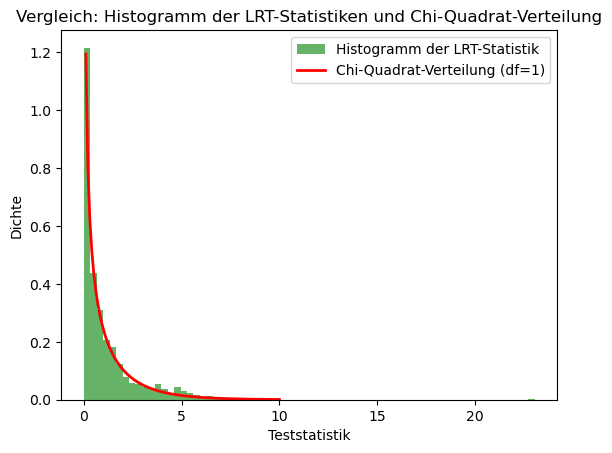
\includegraphics[scale=0.5]{plots/Herzgesundheit_Hist_1000sim_3eff.png}
		\caption{Histogramm der LRT-Statistik mit 1000 Iterationen für gemischte Modelle auf simulierten Daten}
		\label{fig:HIST_MM}
	\end{subfigure}
	\hfill
	\begin{subfigure}[b]{0.5\textwidth}
	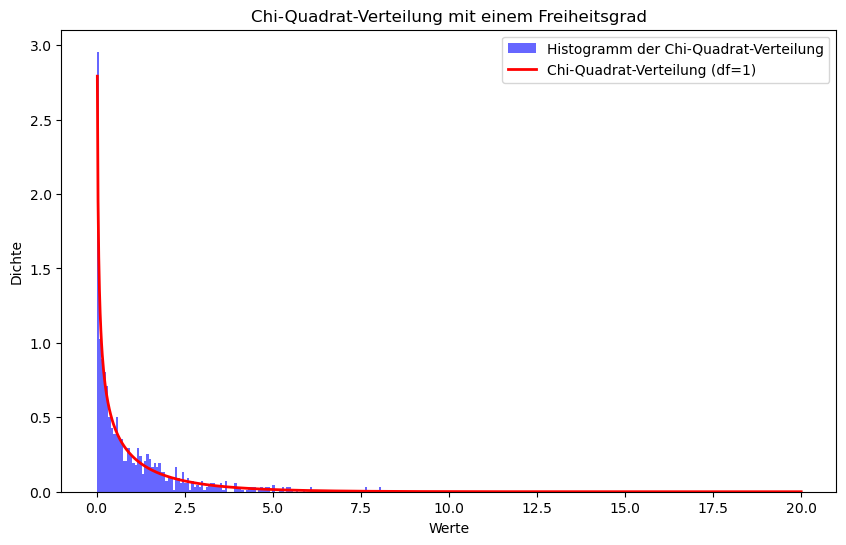
\includegraphics[scale=0.4]{plots/Hist_chi_quadrat.png}
	\caption{Histogramm einer Chi-Quadrat-Verteilung für eine Stichprobengröße von 1000}
	\label{fig:HIST_CHISQUARED}
	\end{subfigure}
	\caption{Histogramme für die LRT-Statistik auf simulierten Daten und einer Chi-Quadrat-Verteilung zum Vergleich}
	\label{HIST2}
\end{figure}

\subsection{Gemischte Modelle in latenten Repräsentationen}
In der bisherigen Betrachtung wurden die gemischten Modelle lediglich auf Basis der tatsächlichen Daten evaluiert. Im Folgenden wird nun die Betrachtung der gemischten Modelle auf latenten Daten vorgenommen. Zur Analyse der gemischten Modelle auf latenten Daten wird das eingeführte Variational-Autoencoder Modell verwendet. Die Grundlage unserer Analyse bildet das folgende Szenario: \\
\\
Zur Analyse wird nun ein komplexer longitudinaler medizinischer Datensatz betrachtet, der durch einen Encoder des VAEs im latenten Raum modelliert wird. Das Ziel ist es nun, das reduzierte und das vollständige gemischte Modell auf dieser latenten Datenwolke zu trainieren, um herauszufinden, ob es zu einer erwartbaren Verzerrung kommt. Für das vollständige gemischte Modell wird dem reduzierten Modell ein fester Effekt ohne Einfluss auf die Testergebnisse hinzugefügt. Dazu wird im Folgenden zuerst eine detaillierte Betrachtung des vorliegenden Datensatzes vorgenommen.
\subsubsection{Der Datensatz}
Im Rahmen dieser Bachelorarbeit basieren die Ergebnisse und Experimente, um die Verzerrung der Inferenz bei der Anwendung gemischter Modelle in latenten Repräsentationen zu untersuchen, auf einem generierten, hoch-dimensionalen, medizinischem Datensatz, welcher sich aus drei zentralen Datensätzen zusammensetzt. Diese Datensätze enthalten Informationen über die Basisdaten der Patienten, die Testergebnisse der Patienten und zeitbezogene Informationen zu jedem Patienten. Zusammen ergeben sie einen komplexen Datensatz, welcher für 260 Patienten die Ergebnisse von 33 Mobilität-Tests enthält, die mehrmals wiederholt wurden. Somit lässt sich aus diesem Datensatz der Verlauf und die Schwere der Krankheit für jeden Patienten ablesen.  Der Datensatz wurde aus datenschutzrechtlichen Gründen einem originellen Datensatz nachgebaut und bildet die Grundlage der Analyse dieser Arbeit.\\
\\
Im Folgenden wird der komplexe medizinische Datensatz, der für die Hauptanalyse dieser Arbeit verwendet wurde, genauer beschrieben. Er setzt sich aus drei verschiedenen Datensätzen, welche die Basisdaten, die Testergebnisse und die zeitbezogenen Daten enthalten, zusammen. \\
\\
\textbf{Basisdaten}\\
Der 'baseline\_df' Datensatz enthält die grundlegenden Informationen der Patienten, welche mit einer eindeutigen Patienten-ID identifiziert werden. Zu jeder Patienten-ID sind folgenden Informationen gegeben: 
\begin{enumerate}
	\item 'family\_affected': Gibt an, ob die Familie vorerkrankt ist.
	\item 'sco\_surg': Chirurgischer Score.
	\item  '$\leq3$': binäres Merkmal.
	\item 'onset\_age': Alter bei Eintritt der Krankheit.
	\item 'presym\_diag': Prä-symptomatische Diagnose (1: Ja, 0: Nein).
	\item 'presymptomatic': Prä-symptomatischer Zustand (1: Ja, 0: Nein).
	\item 'stand\_lost': Gibt an, ob Patient Stehfähigkeit verloren hat (1: Ja, 0: Nein).
	\item 'stand\_gained': Gibt an, ob Patient Stehfähigkeit gewonnen hat (1: Ja, 0: Nein).
	\item 'stand\_never': Gibt an, ob Patient jemals stehen konnte (1: Ja, 0: Nein).
	\item 'patient\_id': Eindeutige Patienten-ID.
\end{enumerate}
Eine beispielhafter Eintrag im Datensatz ist in Tabelle \ref{table:baseline_df} wiedergegeben. \\
\begin{table}[ht]
	\centering
	\resizebox{\textwidth}{!}{%
		\begin{tabular}{|c|c|c|c|c|c|c|c|c|c|}
			\hline
			patient\_id  & sco\_surg & $\leq$3 & onset\_age & presym\_diag & presymptomatic & stand\_lost & stand\_gained & stand\_never & family\_affected \\
			\hline
			0 & 0.0 & 1.0 & 0.039397 & 1.0 & 0.0 & 0.0 & 0.0 & 1.0 & 1.0 \\
			1 & 0.0 & 0.0 & 2.787249 & 0.0 & 0.0 & 0.0 & 1.0 & 0.0 & -1.0 \\
			2 & 1.0 & 1.0 & 1.471984 & 0.0 & 0.0 & 0.0 & 0.0 & 1.0 & 0.0 \\
			3 & 0.0 & 1.0 & 1.092828 & 0.0 & 0.0 & 0.0 & 0.0 & 1.0 & -1.0 \\
			4 & 0.0 & 0.0 & 13.150771 & 0.0 & 0.0 & 0.0 & 1.0 & 0.0 & -1.0 \\
			\hline
		\end{tabular}
	}
	\caption{Basisdaten der Patienten für Patient 0 bis 4 (baseline\_df)}
	\label{table:baseline_df}
\end{table}
\\
\textbf{Testergebnisse}\\
Der Datensatz 'test\_scores' enthält die Ergebnisse von insgesamt 33 Tests, in denen die Patienten einen Score zwischen 1 und 6 erreichen können. Die Spalte eines Patienten besitzt einen Mobilitäts-Wert und zu jedem Test einen Eintrag (vgl. \ref{table:test_scores}).\\
\begin{table}[ht]
	\centering
	\small
	\begin{tabular}{|c|c|c|c|c|c|c|c|c|c|c|}
		\hline
		patient\_id & mobility & test1 & test2 & test3 & test4 & test5 & test6 & test7 & test8 & ... \\
		\hline
		0 & 3 & 2 & 2 & 2 & 2 & 2 & 2 & 2 & 2 & ... \\
		0 & 6 & 2 & 2 & 2 & 2 & 2 & 2 & 2 & 2 & ... \\
		0 & 6 & 2 & 2 & 2 & 2 & 2 & 2 & 2 & 2 & ... \\
		0 & 6 & 2 & 2 & 2 & 2 & 2 & 2 & 2 & 2 & ... \\
		0 & 6 & 2 & 2 & 2 & 2 & 2 & 2 & 2 & 2 & ... \\
		\hline
	\end{tabular}
	
	\caption{Testergebnisse von Patient 0 (test\_scores)}
	\label{table:test_scores}
\end{table}
\\
\textbf{Zeitbezogene Daten} \\
Der letzte Datensatz 'time\_df' enthält zeitbezogene Informationen, wie das Alter. Des Weiteren gibt er an, seit wann ein Patient behandelt wird ('since\_medication') und wieviel Zeit nach dem letzten Medikamentenwechsel vergangen ist ('since\_switch'). Symbolisch für den Datensatz werden die Daten für die ersten zwei Patienten in Tabelle \ref{table:time_df} erfasst.\\
\\
\begin{table}[ht]
	\centering
	\small
	\begin{tabular}{|c|c|c|c|}
		\hline
		patient\_id & since\_medication & since\_switch & age \\
		\hline
		0 & 1.467488 & 0.000000 & 4.346177 \\
		0 & 1.793292 & 0.000000 & 4.671981 \\
		0 & 2.447639 & 0.000000 & 5.326328 \\
		0 & 2.773443 & 0.000000 & 5.652132 \\
		0 & 3.214237 & 0.383299 & 6.092926 \\
		\hline
	\end{tabular}
	\caption{Zeitbezogene Daten von Patient 0 (time\_df)}
	\label{table:time_df}
\end{table}
\\
\\
Die Designmatrizen der festen Effekte werden aus dem Basisdatensatz gewonnen, während die Designmatrizen der zufälligen Effekte aus den zeitbezogenen Daten gewonnen werden. Der Datensatz mit den Versuchsergebnissen ist das Rekonstruktionsobjekt, das dem Encoder als Eingangsdaten gegeben wird und das der Decoder so genau wie möglich zu rekonstruieren versucht. Eine genauere Beschreibung der Datensätze findet sich im Anhang.\\
\\
\subsubsection{Gemischtes Modell auf der latenter Datenwolke}
Nachdem der medizinische Datensatz eingeführt wurde, kann die eigentliche Analyse dieser Arbeit beginnen. Das Ziel ist nach wie vor herauszufinden, ob und wie stark es zu einer Verzerrung unter Anwendung gemischter Modelle in latenten Repräsentationen kommt. Ein Testszenario zwischen einem vollständigen und reduzierten gemischten Modell auf den tatsächlichen Daten eines simulierten Datensatzes wurde bereits geschaffen. Nun sollen beide gemischten Modelle auf einer latenten Datenwolke trainiert werden. Wie bereits erwähnt wird im Rahmen dieser Arbeit mit dem bereits eingeführten VAE-Modell gearbeitet. Das gemischte Modell, mit welchem in dieser Arbeit gearbeitet wird, wurde ebenso bereits in Kapitel 1 eingeführt. Allerdings gestalten sich die Designmatrizen abhängig von dem Datensatz, mit dem gearbeitet wird. Deswegen werden die gemischten Modelle nochmal bezüglich des oben beschriebenen Datensatz spezifiziert.\\
\\
\textbf{Das experimentelle Modell}\\
Die Berechnung der Schätzer erfordert die Designmatrizen für die festen und zufälligen Effekte. \\
Der vorgestellte Datensatz umfasst eine Reihe von festen Effekten, die in Tabelle \ref{table:baseline_df} aufgeführt sind. Zusätzlich wurde ein künstlich hinzugefügter Parameter namens 'Geschlecht' integriert. Die Designmatrix der festen Effekte für das vollständige gemischte Modell $X_{full}$ ergibt sich aus den Werten der festen Effekte setzt sich die Designmatrix der festen Effekte. Dementsprechend setzt sich die Designmatrix für die festen Effekte des reduzierten Modells $X_{red}$ lediglich aus den Effekten aus Tabelle \ref{table:baseline_df} zusammen.\\
Die Designmatrizen für die zufälligen Effekte $W_{full}, W_{red}$ beider Modelle basieren auf den Werten der zufälligen Effekte 'since\_medication', 'since\_switch' und 'intercept' zusammen. Da keine Unterschiede zwischen ihnen bestehen, werden sie gemeinsam als $W$ bezeichnet.\\ 
Im vorliegenden Szenario wird der Antwortvektor nicht, wie im gemischten Modell berechneten, verwendet, sondern, wie in Gleichung \ref{MM-auf-latentData} beschrieben, durch die aus dem Encoder gewonnene latente Datenwolke.\\
\\
Für das erste Szenario, was im Rahmen dieser Arbeit untersucht wird, gibt es mehrere Trainingsschritte, die in Algorithmus \ref{Algo1} dargestellt sind. In diesem Szenario wird ein gemischtes Modell auf dem latenten Output eines Variational Autoencoder trainiert. Im ersten Schritt des Trainingsalgorithmus wird der VAE mit der train\_vae Funktion trainiert, welche die normale Loss-Funktion $\mathcal{L}(\alpha=1,\gamma=1) $ maximiert. Im Rahmen des Trainings des Variational Autoencoder wird ein Minibatch-Training verwendet. Diese Methode ermöglicht ein effizientes Training generativer Modelle auf großen Datensätzen. Dazu wird der Datensatz in kleine, handhabbare Teilmengen, sogenannte Minibatches, aufgeteilt. Eine detaillierte Erläuterung des Minibatch-Trainings kann dem Anhang entnommen werden. Im Anschluss wird die negative Log-Likelihood des vollständigen gemischten Modells mit dem latenten Vektor z und den vollständigen Designmatrizen $X_{full}$ und $W_{full}$ maximiert. Für die Optimierung des gemischten Modells wird der zweite Ordnung Optimierer LBFGS gewählt, da dieser bei großen Parameterräumen eine höhere Effizienz aufweist und die Berechnung somit schneller abläuft. Sowohl für das vollständige als auch für das reduzierte gemischte Modell wurde der Optimierer wie folgt initialisiert:
\begin{enumerate}
	\item lr = 0.01 (Lernrate)
	\item max\_iter = 200 (maximale Anzahl an Iterationen pro Optimierungsschritt)
	\item max\_eval = 500 (maximale Anzahl von Funktionsauswertungen pro Optimierungsschritt)
	\item tolerance\_grad = 1e-09 (Abbruchtoleranz bei Optimalität erster Ordnung)
	\item tolerance\_change = 1e-11 (Abbruchtoleranz bei Änderung von Funktionswerten/Parametern)
	\item history\_size = 200 (Größe der Update-Historie)
\end{enumerate}
Mit dieser Initialisierung werden numerische Fehler während der Berechnung verhindert.
Für den Variational Autoencoder fällt die Wahl auf den für tiefe neuronale Netzwerke effizienten ADAM-Optimierer, bei dem nur die Lernrate auf 0.01 angepasst wird. Ansonsten wird mit der Standardinitialisierung gearbeitet.\\
Im zweiten Trainingsschritt wird nun der VAE mit der Funktion train\_vae\_2 trainiert. Diese berücksichtigt den Mean-Squarred-Error und die negative Log-Likelihood in der Loss-Funktion $\mathcal{L}(\alpha=1,\gamma=1,\eta=10,\lambda=10)$. Der Einfluss des Mean-Squared-Error und der negativen Log-Likelihood ist demnach in der Loss-Funktion sehr hoch gewichtet, was das VAE-Modell dazu veranlassen könnte, zu gut zu lernen und somit in der Inferenz eine Verzerrung zu verursachen. Im Anschluss an das zweite Training des Variational Autoencoder wird wieder das vollständige gemischte Modell wie zuvor trainiert. Der zweite Trainingsschritt wird dann insgesamt für 30 Mal wiederholt. Sobald dieser zweite Trainingsschritt abgeschlossen ist, wird dann das reduzierte Modell ein weiteres Mal auf dem zuletzt berechneten latenten Vektor trainiert, wie zuvor das vollständige gemischte Modell.\\
Die zuletzt berechnete negative Log-Likelihood des vollständigen Modells $\mathbf{L}_{full}$ und der negative Log-Likelihood-Wert des reduzierten Modells $\mathbf{L}_{red}$ werden letztendlich mit dem \\ Likelihood-Ratio-Test $LRT(\mathbf{L}_{full},\mathbf{L}_{red})$ ausgewertet. Der Algorithmus \ref{Algo1} wurde für 1000 Wiederholungen durchgeführt und die Ergebnisse $\mathcal{D}_1$ in einem Histogramm in Abbildung \ref{fig:HIST_1latent_dim} gesammelt. Einzelne unplausible Ergebnisse, wie beispielsweise negative Werte, wurden für die Ergebnisse nicht berücksichtigt. Solche Werte können aufgrund von numerischer Instabilität immer vorkommen und verfälschen die Resultate nicht. Für den visuellen Vergleich wurde die Verteilung der beobachteten Daten (in Grün) mit der $\chi^2$-Verteilung mit einem Freiheitsgrad (in Rot) abgeglichen. Wie aus der Abbildung ersichtlich, lässt sich eine gewisse Ähnlichkeit zwischen dem Histogramm \ref{fig:HIST_CHISQUARED} einer $\chi^2$-Verteilung mit einem Freiheitsgrad und dem beobachteten Histogramm \ref{fig:HIST_1latent_dim} feststellen. Um die visuellen Resultate einer numerischen Überprüfung zu unterziehen, wurde der in \ref{Chi-Quadrat-Test} beschriebene Chi-Quadrat-Test auf die beobachteten Daten und eine $\chi^2$-Verteilung mit einem Freiheitsgrad angewendet. Die Daten wurden dabei in zehn Klassen (Bins) unterteilt. Für die anschauliche Darstellung wurden in Abbildung \ref{fig:HIST_1latent_dim} die Daten in 120 Klassen unterteilt. Für den numerischen Test könnte dies allerdings zu Verfälschungen der Ergebnisse führen.\\
Die Hypothesen für das erste Testszenario lauten:\\
\begin{enumerate}
	\item Nullhypothese ($\mathbf{H}_0$): Die Daten $\mathcal{D}_1$ folgen der $\chi^2$-Verteilung mit einem Freiheitsgrad\\
	\item Alternativhypothese ($\mathbf{H}_1$): Die Daten $\mathcal{D}_1$ folgen nicht der $\chi^2$-Verteilung mit einem Freiheitsgrad \\
\end{enumerate}
Das Signifikanzniveau wird auf 5 \% gesetzt ($\alpha_0 = 0.05$).
Für die beobachteten Daten $\mathcal{D}_1$ des ersten Testszenarios ist der Wert des Chi-Quadrat-Test folgendermaßen:\\
$$\mathcal{X}^2_1 = 0.05157511461061281$$
Um zu testen, ob die Nullhypothese angenommen wird, benötigt es noch den Wert des (1-$\alpha_0$)-Quantils einer $\chi^2$-Verteilung mit einem Freiheitsgrad.\\
Dieser Wert $\chi^2_{(1-\alpha_0; 1)} = 3.841458820694124$ ist folglich der kritische Wert.
Die Nullhypothese wird demnach angenommen, da $$0.05157511461061281 < 3.841458820694124$$ gilt. Somit wurde auch numerisch bestätigt, dass die Verteilung der Daten einer $\chi^2$-Verteilung mit einem Freiheitsgrad folgt. 
\\
Für dieses Testszenario ist demnach eine Verzerrung in der Inferenz weder zu erkennen noch zu messen. Dies bedeutet, dass der Mean Squarred Error und die negative Log-Likelihood trotz hoher Gewichtung in der Loss-Funktion keinen Einfluss auf das Training des Variational Autoencoder haben und der Encoder nicht zu gut lernt.\\
\\
\textbf{Gemischtes Modell auf latenter Datenwolke eines Autoencoders}\\
In einem zweiten Szenario, was im Rahmen dieser Arbeit untersucht wurde, wurde das VAE-Modell durch einen üblichen Autoencoder ausgetauscht. Die Anpassung ist relativ einfach zu bewerkstelligen, da lediglich der Output des Encoders verwendet wird und somit der Reparametrisierungstrick weggelassen wird. Die latenten Variablen sind dann einfach $\mu$, wie sie oben für das VAE-Modell vorgestellt wurden. Im Gegensatz zu Variational Autoencodern, welche die Eingabedaten als Verteilung kodieren, kodiert ein üblicher Autoencoder die Eingabedaten in einem festen latenten Raum. Dies resultiert in einer zu starken Adaption spezifischer Merkmale der Trainingsdaten durch das Modell. Die Reduzierung des Variational Autoencoder zu einem normalen Autoencoder führt folglich zu einer erhöhten Anfälligkeit für Overfitting. Im Algorithmus \ref{Algo1} sind lediglich Anpassungen der train\_vae und train\_vae\_2 Funtkion erforderlich, um eine neue LRT-Statistik zu erhalten, welche in Abbildung \ref{fig:HIST_Autoencoder} dargestellt ist. Die beobachteten Daten $\mathcal{D}_2$ aus dem zweiten Testszenario wurden wiederum für den visuellen Vergleich in 120 Klassen unterteilt und mit einer $\chi^2$-Verteilung abgeglichen. Einzelne unplausible Ergebnisse in $\mathcal{D}_2$ wurden für die Auswertung  erneut ignoriert. Auch für dieses Szenario ist in Abbildung \ref{fig:HIST_Autoencoder} keine Verzerrung zu erkennen. Für die numerische Überprüfung dieser Vermutung werden die Hypothesen wie folgt aufgestellt:\\
\begin{enumerate}
	\item Nullhypothese ($\mathbf{H}_0$): Die Daten $\mathcal{D}_2$ folgen der $\chi^2$-Verteilung mit einem Freiheitsgrad\\
	\item Alternativhypothese ($\mathbf{H}_1$): Die Daten $\mathcal{D}_2$ folgen nicht der $\chi^2$-Verteilung mit einem Freiheitsgrad \\
\end{enumerate}
Das Signifikanzniveau $\alpha_0$ und der kritische Wert $\chi^2_{(1-\alpha_0; 1)}$ ändern sich nicht im Vergleich zu dem ersten Testszenario.
Berechnet man nun die Chi-Quadrat-Statistik, wie in \ref{Chi-Quadrat-Test} beschrieben, so erhält man den Wert $\mathcal{X}^2_2 = 0.04330499004467964 < \chi^2_{(1-\alpha_0; 1)}$. Die Nullhypothese wird demnach auch im zweiten Testszenario angenommen. Wie der visuellen Darstellung zu entnehmen ist, kommt es bei der Reduzierung des VAE-Modells zu keiner Verzerrung, wenn ein herkömmlichen Autoencoder verwendet wird. \\
\\
\begin{figure}[h]
	\centering
	\begin{subfigure}[b]{0.45\textwidth}
		\centering
		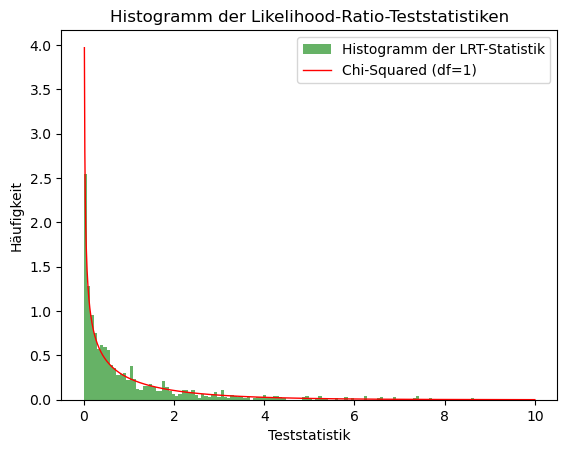
\includegraphics[width=\textwidth]{plots/1_latent_dim_VAE.png}
		\caption{Histogramm der LRT-Statistik mit 1000 Iterationen für gemischte Modelle auf latenter Datenwolke eine einfachen VAE-Modells}
		\label{fig:HIST_1latent_dim}
	\end{subfigure}
	\hfill
	\begin{subfigure}[b]{0.45\textwidth}
		\centering
		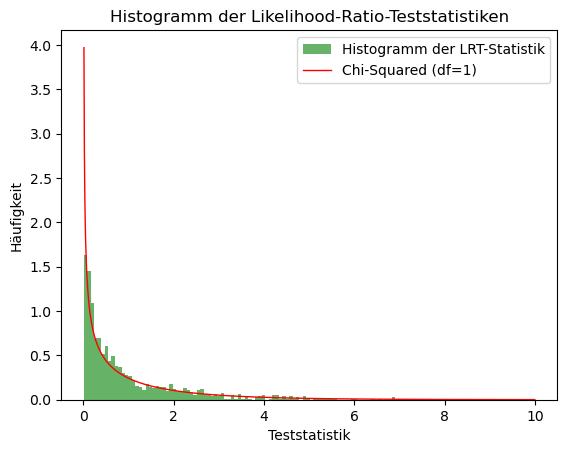
\includegraphics[width=\textwidth]{plots/Autoencoder.png}
		\caption{Histogramm der LRT-Statistik mit 1000 Iterationen für ein gemischtes Modell auf latenter Datenwolke eines Autoencoders}
		\label{fig:HIST_Autoencoder}
	\end{subfigure}
	\caption{Histogramme der LRT-Statistiken mit einer Unterteilung in 120 Klassen}
	\label{fig:LRT_HIST2}
\end{figure}
\\
\textbf{Gemischtes Modell auf der latenten Datenwolke eines komplexen VAE-Modells}\\
In einem letzten dritten experimentellen Szenario wird die Komplexität des Encoder-Modells erhöht. Das Ziel ist es wieder ein "Overfitting" zu provozieren. Im zuerst vorgestellten Szenario wurde mit dem eingeführten VAE-Modell gearbeitet. In dem bereits vorgestellten Modell verfügt der Encoder über eine versteckte Schicht mit 150 Neuronen, welche die Eingabedaten in einen eindimensionalen latenten Raum transformiert. Um die Komplexität des Encoder-Modells zu erhöhen wird dem Encoder nun eine zusätzliche versteckte Schicht hinzugefügt und die Anzahl der Neuronen wird auf 200 erhöht. Die Anzahl der Dimensionen im latenten Raum wird insbesondere auf vier erhöht, was eine Erhöhung der Komplexität des Modells zur Folge hat. Im Rahmen dieses neuen Encoder-Modells wird der Algorithmus \ref{Algo1} für eine weitere LRT-Statistik ausgeführt. Die so gewonnenen Daten $\mathcal{D}_3$, welche keine einzelnen negativen Werte enthalten, welche wiederum ignoriert wurden, sind in Abbildung \ref{fig:HIST_4latentdim} als Histogramm mit 120 Klassen dargestellt. Das Histogramm weist in diesem Szenario eine starke Verzerrung auf und erweckt den Anschein, dass es nicht mehr einer $\chi^2$-Verteilung folgt. Bei einer  Überanpassung kann die Wahrscheinlichkeit des komplexeren VAE-Modells (mit 4 latenten Dimensionen) für die Trainingsdaten unverhältnismäßig hoch sein, was zu größeren Werten der Teststatistik führt. Daher ist im Histogramm \ref{fig:HIST_4latentdim} eine breitere Streuung zu sehen. Zur numerischen Überprüfung werden ein letztes Mal die Hypothesen aufgestellt. \\
\begin{enumerate}
	\item Nullhypothese ($\mathbf{H}_0$): Die Daten $\mathcal{D}_3$ folgen der $\chi^2$-Verteilung mit einem Freiheitsgrad\\
	\item Alternativhypothese ($\mathbf{H}_1$): Die Daten $\mathcal{D}_3$ folgen nicht der $\chi^2$-Verteilung mit einem Freiheitsgrad \\
\end{enumerate} 
Das Ergebnis des Chi-Quadrat-Tests ergibt einen Wert von
$\mathcal{X}^2_2 = 0.7768478802621662$. Der Wert liegt zwar leicht über dem der vorherigen Werten, jedoch immer noch unter dem kritischen Wert $\chi^2_{(1-\alpha_0; 1)}$. Dies impliziert, dass die Nullhypothese auch im letztem Szenario mit einer erkennbaren Verzerrung angenommen wird. Die Histogramme der Chi-Quadrat-Tests für alle drei Szenarien mit nur zehn Klassen sind im Anhang zu finden. \\
\\
\begin{figure}[H]
	\centering
	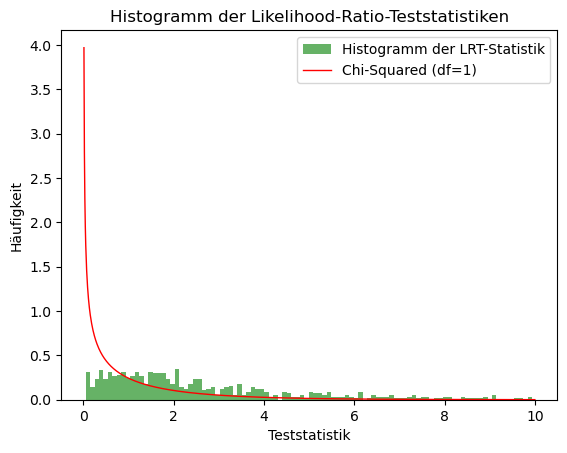
\includegraphics[scale=0.6]{plots/4_latent_dim_VAE.png}
	\caption{Histogramm der LRT-Statistik mit 1000 Iterationen für gemischte Modelle auf latenter Datenwolke eines komplexen VAE-Modell}
	\label{fig:HIST_4latentdim}
\end{figure}
\begin{algorithm}[h]
	\SetAlgoLined
	\KwData{num\_simulations = 1000, iterations = 30, $X_{\text{full}}$, $W_{\text{full}}$, $X_{\text{red}}$, $W_{\text{red}}$}
	\KwResult{lrt\_results}
	\SetKw{Initialize}{Initialize}
	\SetKw{Train}{train\_vae}
	\SetKw{TrainTwo}{train\_vae\_2}
	\SetKw{Calc}{calc\_likelihood}
	\SetKw{Likelihood}{likelihood\_ratio}
	\SetKw{Maximize}{maximize}
	\SetKw{Calculate}{calculate}
	\SetKw{Update}{update}
	
	\For{$i \gets 1$ \textbf{to} num\_simulations}{
		Load and prepare datasets\;
		\Initialize{$encoder$, $decoder$} \;
		\Initialize{$optimizer\_vae(encoder.parameters(),decoder.parameters())$}\;
		$z \gets \Train(epochs=2, batch\_size=128, encoder, decoder)$\;
		
		\For{$j \gets 0$ \textbf{to} iterations}{
			\If{$j \neq 0$}{
				$z \gets \TrainTwo(epochs=1, batch\_size=128, encoder, decoder, optimizer\_vae, W_{\text{full}}, X_{\text{full}}, Q_{\text{full}}, R_{\text{full}})$\;
			}
			\Initialize{$Q_{\text{full}}, R_{\text{full}}$}\;   
			\Initialize{$optimizer\_mm\_full(Q_{\text{red}}, R_{\text{red}})$}      
			\Maximize{$l_{\text{ML}}(Q_{\text{full}}, R_{\text{full}})$} $\gets X_{\text{full}}, W_{\text{full}}, z$\;
		}
		
		\Initialize{$Q_{\text{red}}, R_{\text{red}}$}\;     
		\Initialize{$optimizer\_mm\_full(Q_{\text{red}}, R_{\text{red}})$}   
		\Maximize{$l_{\text{ML}}(Q_{\text{red}}, R_{\text{red}})$} $\gets X_{\text{red}}, W_{\text{red}}, z$\;
		
		$res_{\text{full}} \gets l_{\text{ML}}(Q_{\text{full}}, R_{\text{full}})$\;
		$res_{\text{red}} \gets l_{\text{ML}}(Q_{\text{red}}, R_{\text{red}})$\;
		
		$lrt\_val \gets \Likelihood(res_{\text{full}}, res_{\text{red}})$\;
		$lrt\_results$ add $lrt\_val$\;
	}
	
	\caption{Algorithmus zur Simulation und Berechnung der Likelihood-Ratio-Teststatistik aus Experiment 1}
	\label{Algo1}
\end{algorithm}
\subsection{Post-Selection-Inferenz (PSI)}
Dieser Abschnitt gibt einen kurzen Überblick über einen vielversprechenden Ansatz zur weiteren Untersuchung von Inferenzverzerrungen, die Post-Selection Inference (PSI).\\
\\
\textbf{Einführung}\\
Post-Selection-Inferenz (PSI) ist eine statistische Methode, die darauf abzielt, die Verzerrungen zu korrigieren, die nach der Modellauswahl auftreten können. Wie man gesehen hat kann die Wahl eines komplexeren Modells zu einer systematischen Verzerrung der Inferenz führen.\\
\\
PSI berücksichtigt diese Modellauswahl und bietet Methoden zur Korrektur der dadurch entstehenden Verzerrungen. Insbesondere bei komplexen Modellen wie Variational Autoencoders (VAE) in Kombination mit gemischten Modellen ist die Berücksichtigung der Modellauswahl von entscheidender Bedeutung, um zuverlässige und gültige Schlussfolgerungen ziehen zu können.\\
\\
\textbf{Prinzipien der Post-Selection-Inferenz}\\
PSI basiert auf der Idee, die Unsicherheit der Modellauswahl explizit in die Inferenz einzubeziehen. Dies wird durch Konditionierung auf die Modellauswahl oder Anpassung der Teststatistiken erreicht.\\
\begin{enumerate}
\item{Konditionierung auf die Modellauswahl:}\\
Anstatt die Inferenz auf dem ausgewählten Modell durchzuführen, wird die Unsicherheit, die durch den Auswahlprozess entsteht, konditioniert. Dies bedeutet, dass die Schätzungen und Tests die Tatsache berücksichtigen, dass das Modell aus einer Menge möglicher Modelle ausgewählt wurde.\\
\item{Anpassung der Teststatistiken:}\\
Die Teststatistiken und Konfidenzintervalle werden angepasst, um die zusätzlichen Freiheitsgrade, die durch die Modellauswahl entstehen, zu berücksichtigen. Dadurch werden konservativere und weniger verzerrte Schätzungen erzielt.\\
\end{enumerate}
\textbf{Anwendungen der Post-Selection-Inferenz}\\
Die Anwendung von PSI in der Kombination von VAEs und gemischten Modellen kann mehrere Vorteile bieten.
\\
\begin{enumerate}
	\item{Verbesserte Zuverlässigkeit der Inferenz:}\\
	Durch die Berücksichtigung der Modellauswahlprozesse kann die Verzerrung der Inferenz reduziert werden, was zu verlässlicheren und stabileren Ergebnissen führt.\\
	\item{Genaue Konfidenzintervalle:}\\
	PSI bietet genauere Konfidenzintervalle für die Modellparameter, die die Unsicherheit der Modellauswahl korrekt widerspiegeln.\\
	\item{Bessere Modellbewertung:}\\ 
	Die Anpassung der Teststatistiken ermöglicht eine genauere Bewertung der Modellgüte und eine verbesserte Entscheidungsfindung bei der Auswahl des besten Modells.
\end{enumerate}

\section{Interpretation der Ergebnisse}
In dem vorangegangenen Kapitel wurde versucht das experimentelle Modell zu einem sogenannten 'Overfitting' zu zwingen. Dabei wurde der Loss-Funktion des Variational Autoencoder in einem ersten Experiment der Mean Squarred Error und die negative Log-Likelihood des vollständigen gemischten Modell hinzugefügt. Somit wurde der Variational Autoencoder provoziert zu gut vom gemischten Modell zu lernen. Zudem wurde der Variational Autoencoder in einem weiterem Experiment zu einem herkömmlichen Autoencoder reduziert, wodurch das Modell an Stabilität verloren hat. Durch die Reduzierung zu einem herkömmlichen Autoencoder geht die Eigenschaft verloren, dass der Autoencoder eine Verteilung lernt und es war erwartbar, dass somit zu viele Details aus dem Datensatz gelernt werden. In einem letztem Experiment wurde in den Variational Autoencoder aus dem ersten Szenario eine zusätliche Encoder Schicht hinzugefügt und die latente Dimension auf vier erhöht. Die Komplexität des so entstandenen Modells wurde dadurch erhöht und ein Overfitting noch mehr provoziert. Die Komplexität des Modells kann dazu führen, dass das Modell die Trainingsdaten zu gut anpasst und somit auch das Rauschen erfasst.\\
\\
Die Ergebnisse der drei Testszenarios wurden in Form von Histogrammen in Abbildung \ref{fig:HIST_4latentdim} und \ref{fig:LRT_HIST2} zusammengetragen. Die Histogramme liefern einen visuellen Abgleich mit der $\chi^2$-Verteilung. Da dies alleine allerdings kein zuverlässiger Beleg wäre, wurden die Ergebnisse zudem noch numerisch anhand des Chi-Quadrat-Test überprüft. Insbesondere wurde zum visuellen Abgleich ein einfaches Szenario geschaffen, in dem zwei gemischte Modelle auf den tatsächlichen Daten eines simulierten Datensatzes trainiert wurden. In diesem Szenario war die in Abbildung \ref{fig:HIST_MM} dargestellte $\chi^2$-Verteilung der LRT-Statistik zu erwarten. Wie man sieht folgt das grüne Histogramm ohne Verzerrung der roten Kurve, welche die $\chi^2$-Verteilung beschreibt. Dies bedeutet, dass bis auf einzelne Ausnahmen, welche durch Instabilitäten der Berechnung immer verursacht werden können, die Ergebnisse des LRT-Statistik einer $\chi^2$-Verteilung mit einem Freiheitsgrad folgen.\\
\\
Wenn man nun die Histogramme in \ref{fig:LRT_HIST2} und das Histogramm in \ref{fig:HIST_MM} vergleicht, ist kaum ein Unterschied zu erkennen. Es lässt sich also vermuten, dass die Histogramme einer $\chi^2$-Verteilung ohne Verzerrung folgen. Diese Vermutung wurde zudem numerisch anhand des Chi-Quadrat-Tests belegt. Für die Anwendung gemischter Modelle in der latenten Repräsentation eines einfachen Variational Autoencoder Modells liegt also keine Verzerrung der Inferenz vor. Somit kann die dimensionsreduzierte Darstellung von mehrdimensionalen Datensätzen durch einfache VAE-Modelle für die Anwendung gemischter Modelle ohne Verlust von Validität ausgenutzt werden. Dies ist bereits eine große Erleichterung bei der Analyse komplexer Datensätze anhand gemischter Modelle, da so der Handhabung solcher Datensätze bedeutend erleichtert wird. Auch die latente Repräsentation einfacher Autoencoder-Modelle kann für die dimensionsreduzierte Darstellung hochdimensionaler Datensätze ausgenutzt werden. \\
\\
Allerdings sollte man dies mit Vorsicht genießen. Wenn man die Histogramme in Abbildung \ref{fig:HIST_4latentdim} und Abbildung \ref{fig:HIST_CHISQUARED} vergleicht, kommt man leicht auf die Vermutung, dass die Teststatistik aus dem dritten Experiment nicht mehr einer $\chi^2$-Verteilung mit einem Freiheitsgrad folgt. Diese Vermutung konnte allerdings  anhand des  Chi-Quadrat-Tests nicht bestätigt werden. Wie man visuell erkennen kann und wie auch der etwas erhöhte Wert des Chi-Quadrat-Tests zeigt, gibt es also eine Verzerrung der Inferenz bei der Verwendung komplexerer VAE-Modelle. Der numerische Test zeigt, dass die Verzerrung, die sich in einem höheren Wert des Tests zeigt, noch innerhalb des Signifikanzniveaus liegt. Die erkennbare Verzerrung ist demnach akzeptabel und die Teststatistik folgt einer $\chi^2$-Verteilung. Die Teststatistik in Abbildung \ref{fig:HIST_4latentdim} des komplexeren VAE-Modells sieht zwar dramatischer aus, als sie numerisch bestätigt werden konnte, ist jedoch nicht zu Vernachlässigen. Auch diese akzeptable Verzerrung kann die Ergebnisse schon beeinflussen. Die kurz eingeführte Methode Post-Selection-Inferenz kann dabei in Zukunft eine vielversprechende Methode sein, um die Verzerrung der Inferenz bei der Wahl komplexerer Modelle zu verringern.
\\
\section{Limitationen und Herausforderungen}
Trotz der zufriedenstellenden Ergebnisse der Arbeit gibt es genug bleibende Herausforderungen und Limitationen. Eines der Größten Risiken bei der Verwendung gemischter Modelle in latenten Repräsentationen ist das Risiko der Überanpassung. Wenn das Modell sich zu gut an den Trainingsdatensatz anpasst, birgt dies das Risiko zu gut von diesem zu Lernen und somit auch das Rauschen zu lernen. Dies führt zu einer schlechteren Generalisierung auf neuen Daten. In den Experimenten wurde deutlich, dass bei nur leicht komplexeren Modellen schon eine Verzerrung der Inferenz sichtbar ist. Zwar ist diese noch akzeptabel in ihrer Größe, jedoch wird diese bei noch tieferen neuronalen Netzen noch stärker. Falls es zu Verzerrungen in der Inferenz kommt, kann dies dann zu fehlerhaften Schlussfolgerungen führen. \\
\\
Die Anwendung gemischter Modelle in latenten Repräsentationen reduziert zwar die Dimension der Daten und erleichtert somit deren Handhabung, jedoch erhöht sich der Rechenaufwand solcher Modelle erheblich. Besonders bei komplexeren Modellen ist der Rechenaufwand und der benötigte Speicher sehr hoch, was die Anwendung solcher Modelle einschränken kann. 

\chapter{Fazit}
Diese Arbeit hat die Verzerrung der Inferenz bei der Verwendung gemischter Modelle in latenten Repräsentationen untersucht, insbesondere unter Einsatz von Variational Autoencoder (VAE). Die Ergebnisse zeigen, dass die Kombination von VAEs und gemischten Modellen eine vielversprechende Methode zur Analyse hochdimensionaler Daten ist. Es konnte für einfache Modelle keine Verzerrung in der Inferenz festgestellt werden. Aufgrund dessen kann für einfache Szenarien die Anwendung gemischter Modelle in latenten Repräsentationen empfohlen werden. Allerdings konnte für komplexere Modelle eine Verzerrung in der Inferenz visuell festgestellt werden, wenn das gemischte Modell auf der latenten Datenwolke eines tieferen neuronalen Netzes trainiert wurde. Diese Verzerrung konnte zwar numerisch anhand eines leicht erhöhten Wertes bestätigt werden, ist allerdings immer noch in einem akzeptablen Signifikanzniveau. Trotzdem kann diese Verzerrung zu fehlerhaften Schlussfolgerungen führen und die Validität der Modelle mindern. Die durchgeführten Analysen bieten also wertvolle Erkenntnisse für die Anwendung und Weiterentwicklung dieser Modelle in der Praxis.

\section{Ausblick}
Zukünftige Forschungen sollten die Grenzen der Modelle weiter analysieren und die Verzerrung für noch tiefere neuronale Netze quantifizieren. Insbesondere sollte erforscht werden, inwiefern die akzeptierte Verzerrung die Ergebnisse nicht doch beeinflussen könnte.\\
Darüber hinaus wäre es sinnvoll, die Anwendbarkeit dieser Methoden auf mehreren realen medizinischen Datensätzen zu überprüfen, um deren praktischen Nutzen zu validieren und gegebenenfalls anzupassen. Des Weiteren kann es von Vorteil sein, die Analyse für eine andere latente Repräsentation als Autoencoder oder Variational Autoencoder durchzuführen, um bei der praktischen Anwendung solcher Modelle flexibler zu sein.\\
\\
Für zukünftige Forschungen wird empfohlen, die Verzerrung der Inferenz durch die Integration von Post-Selection-Inferenz (PSI) zu minimieren. Die Integration von PSI in die Analyse von gemischten Modellen in latenten Repräsentationen eröffnet neue Möglichkeiten zur Verbesserung der statistischen Inferenz. In zukünftigen Arbeiten könnte die Anwendung von PSI auf verschiedene Datensätze und Modellkonfigurationen weiter erforscht werden, um die Robustheit und Genauigkeit der Inferenz zu erhöhen. Dies könnte insbesondere in Bereichen wie der medizinischen Datenanalyse, wo präzise und zuverlässige Inferenzmethoden von entscheidender Bedeutung sind, von großem Nutzen sein.
\\
\chapter{Anhang}
\section{Herzgesundheits-Datensatz}
Das Simulationsdesign für den Herzgesundheits-Datensatz wurde bereits in Kapitel 3.2.1 beschrieben. Es folgen Ergänzungen zur Veranschaulichung und zum tieferen Verständnis des Simulationsdesign. Die Trajektorien der festen Effekte 'Systolischer Blutdrck', 'Diastolischer Blutdruck', 'Cholesterinspiegel', Body-Maß-Index' (BMI) und der Testwerte 'Gesundheitsscore' sind in Abbildung \ref{fig:sample_image} für fünf zufällig ausgewählte Patienten dargestellt. Der Wechsel der Farbe einer Trajektorie eines Patienten von Rot auf Grün symbolisiert den Anfang einer Behandlung. Es ist zu erkennen, dass sich mit dem Wechsel der Farben die Werte grundsätzlich verbessern. Dies hängt damit zusammen, dass mit Start der Behandlung die aus den Normalverteilungen (vgl. \ref{tab:health_score_parameters}) gezogenen Daten pro Jahr mit den in Tabelle \ref{tab:weights} dargestellten Werten verbessert werden. Vor der Behandlung werden die Daten mit geringeren Parametern angepasst, was eine minimale natürliche Verbesserung simulieren soll. Die Werte dazu sind genauso wie der Einfluss der festen Effekte auf den Gesundheitsscore in Tabelle \ref{tab:weights} dargestellt. Der Start der Behandlung wird zufällig nach zwischen Jahr drei bis zehn ausgewählt. Für die Berechnung der Testergebnisse in Form des Health-Scores wird ein Startwert von 150 eingesetzt, damit die Ergebnisse stets positiv sind und eine realistischere Studie entsteht. 
\begin{table}[H]
	\centering
	\begin{tabular}{|p{3cm}|p{3cm}|p{3cm}|p{3cm}|}
		\hline
		&  natürliche Verbesserung pro Jahr &  Behandlungseffekt pro Jahr &  Effekt auf den Gesundheitsscore \\
		\hline
		Systolischer Blutdruck & -0.5 &  -2 &  -0.1 \\
		\hline
		Diastolischer Blutdruck &  -0.5 &  -2 &  -0.1 \\
		\hline
		Cholesterin &  -1 &  -5 &  -0.2 \\
		\hline
		Triglycerides &  -1 &  -3 &  -0.2 \\
		\hline
		BMI &  / &  / &  -0.4 \\
		\hline
		Creatinin &  -0.01 &  -0.08 &  -0.1 \\
		\hline
	\end{tabular}
	\caption{Gewichte des Simulationsdesigns des Herzgesundheits-Datensatz}
	\label{tab:weights}
\end{table}
\begin{figure}[H]
	\centering
	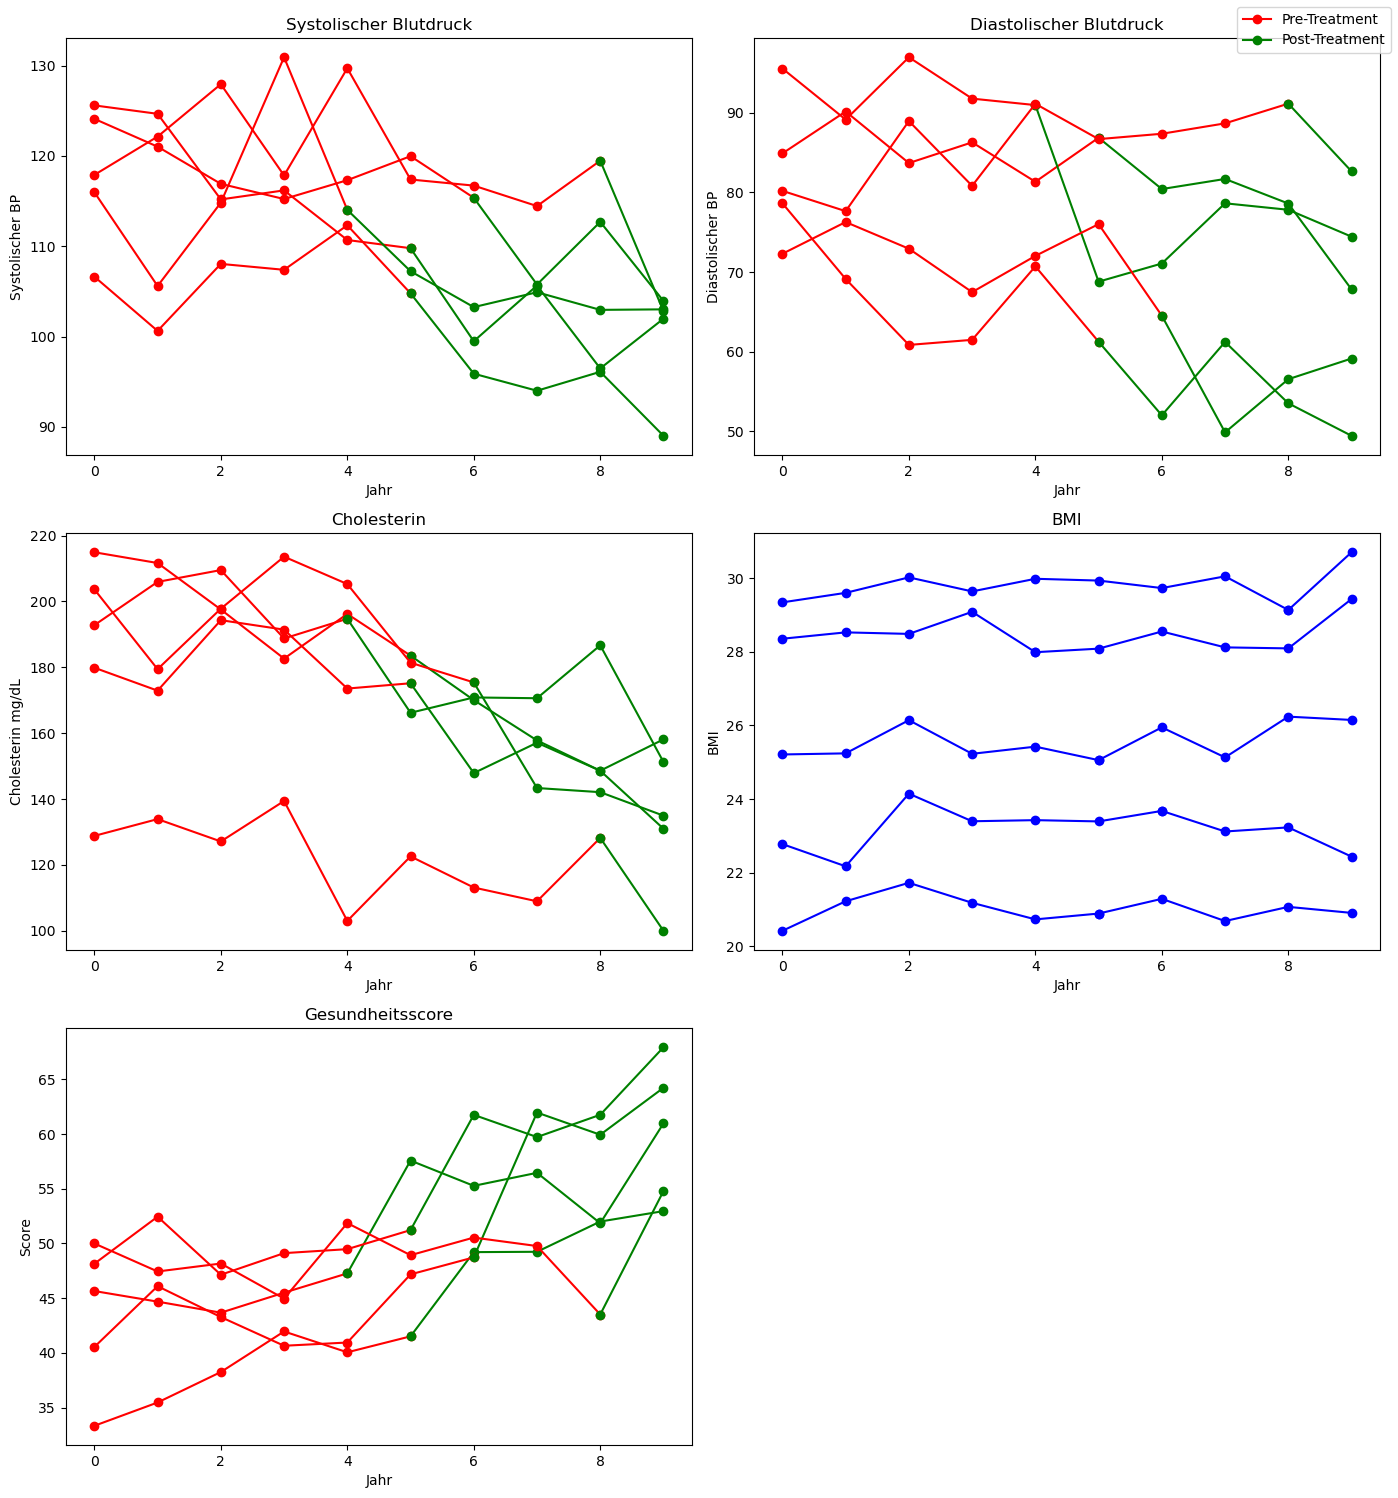
\includegraphics[width=\linewidth]{plots/Herzgesundheit_Datensatz.png}
	\caption{Trajektorien der festen Effekte und des Gesundheitsscores eines simulierten Datensatzes für 20 zufällig ausgewählte Patienten}
	\label{fig:sample_image}
\end{figure}

\section{Histogramme der LRT-Statistiken mit einer Unterteilung in 10 Klassen}
\begin{figure}[H]
	\centering
	\begin{subfigure}[b]{0.45\textwidth}
		\centering
		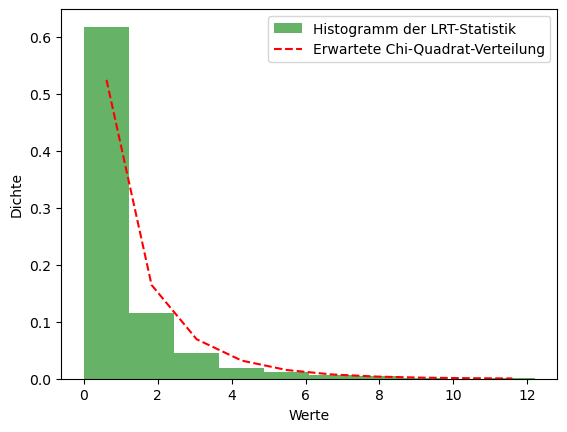
\includegraphics[width=\textwidth]{plots/1_latent_dim_VAE_10bins.png}
		\caption{Histogramm der LRT-Statistik mit 1000 Iterationen für gemischte Modelle auf latenter Datenwolke eines einfachen VAE-Modells}
		\label{fig:HIST_1latent_dim_10bins}
	\end{subfigure}
	\hfill
	\begin{subfigure}[b]{0.45\textwidth}
		\centering
		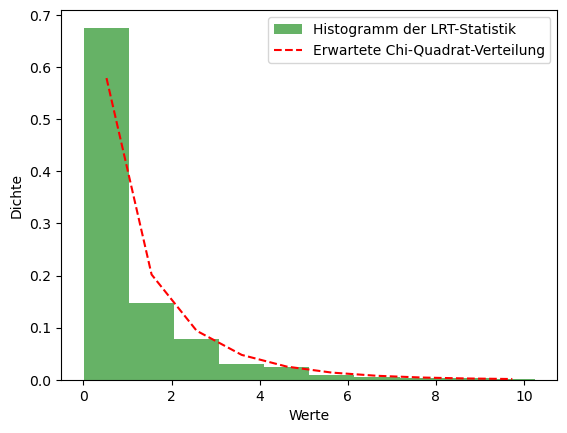
\includegraphics[width=\textwidth]{plots/Autoencoder_10bins.png}
		\caption{Histogramm der LRT-Statistik mit 1000 Iterationen für ein gemischtes Modell auf latenter Datenwolke eines Autoencoders}
		\label{fig:HIST_Autoencoder_10bins}
	\end{subfigure}
	\hfill
		\begin{subfigure}[b]{0.45\textwidth}
		\centering
		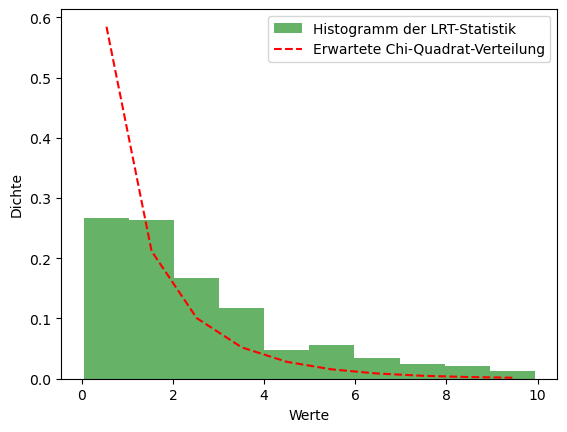
\includegraphics[width=\textwidth]{plots/4_latent_dim_VAE_10bins.png}
		\caption{Histogramm der LRT-Statistik mit 1000 Iterationen für ein gemischtes Modell auf latenter Datenwolke eines komplexen VAE-Modells}
		\label{fig:HIST_4latent_dim_10bins}
	\end{subfigure}
	\caption{Histogramme der LRT-Statistiken mit einer Unterteilung in zehn Klassen}
	\label{fig:LRT_HIST2_10bins}
\end{figure}
\section{Minibatch-Training}
Das Minibatch-Training ist eine Form des Stochastic Gradient Descent (SGD), bei dem die Modellparameter mithilfe kleiner, zufällig ausgewählter Teilmengen des Datensatzes aktualisiert werden, anstatt den gesamten komplexen Datensatz auf einmal zu verwenden. Diese Methode hat mehrere Vorteile. Es reduziert nicht nur den Speicherbedarf, da immer nur kleine Teilmengen der Daten im Speicher geladen werden, sondern ermöglicht gleichzeitig eine schnellere Konvergenz, da die Modellparameter häufiger aktualisiert werden. \\
\\
Im Falle des in dieser Arbeit verwendeten Modells, wird vor der Trainingsschleife der Datensatz für ein Minibatch-Training vorbereitet. Dies geschieht ganz einfach, indem der Datensatz in mehrere Minibatches aufgeteilt wird. Die Größe der Minibatches ist häufig eine Potenz von 2 (z.B. 16, 32, 64, 128)
\backmatter{}
\pagenumbering{arabic}
%\listoffigures% may be removed
%\listoftables% may be removed
%\bibliography{literature.bib}
\printbibliography{} % print bibliography
\chapter{Danksagungen}
An dieser Stelle möchte ich mich recht herzlich bei Herr Clemens Schächter für die stets zuvorkommende und zeitintensive Betreuung bedanken. Ohne den ständigen Austausch und ohne die interessanten Anregungen wäre diese Arbeit mit Sicherheit so nicht zustande gekommen.\\
\\
Außerdem bedanke ich mich recht herzlich bei Prof. Dr. Harald Binder für die sehr angenehme Kooperation und den häufigen fachlichen Austausch. 
\chapter{Erklärung}
Hiermit erkläre ich, dass ich diese Bachelorarbeit eigenständig verfasst habe und keine anderen als
die von mir angegebenen Quellen und Hilfsmittel benutzt habe und dass ich diese Arbeit nicht
bereits zur Erlangung eines akademischen Grades eingereicht habe.
\end{document}

%%% Local Variables:
%%% mode: latex
%%% TeX-engine: default
%%% TeX-command-extra-options: "-shell-escape"
%%% ispell-local-dictionary: "american"
%%% eval: (setenv "TEXINPUTS" ".//:")
%%% TeX-master: t
%%% End:
